% Options for packages loaded elsewhere
\PassOptionsToPackage{unicode}{hyperref}
\PassOptionsToPackage{hyphens}{url}
%
\documentclass[
]{book}
\usepackage{lmodern}
\usepackage{amssymb,amsmath}
\usepackage{ifxetex,ifluatex}
\ifnum 0\ifxetex 1\fi\ifluatex 1\fi=0 % if pdftex
  \usepackage[T1]{fontenc}
  \usepackage[utf8]{inputenc}
  \usepackage{textcomp} % provide euro and other symbols
\else % if luatex or xetex
  \usepackage{unicode-math}
  \defaultfontfeatures{Scale=MatchLowercase}
  \defaultfontfeatures[\rmfamily]{Ligatures=TeX,Scale=1}
\fi
% Use upquote if available, for straight quotes in verbatim environments
\IfFileExists{upquote.sty}{\usepackage{upquote}}{}
\IfFileExists{microtype.sty}{% use microtype if available
  \usepackage[]{microtype}
  \UseMicrotypeSet[protrusion]{basicmath} % disable protrusion for tt fonts
}{}
\makeatletter
\@ifundefined{KOMAClassName}{% if non-KOMA class
  \IfFileExists{parskip.sty}{%
    \usepackage{parskip}
  }{% else
    \setlength{\parindent}{0pt}
    \setlength{\parskip}{6pt plus 2pt minus 1pt}}
}{% if KOMA class
  \KOMAoptions{parskip=half}}
\makeatother
\usepackage{xcolor}
\IfFileExists{xurl.sty}{\usepackage{xurl}}{} % add URL line breaks if available
\IfFileExists{bookmark.sty}{\usepackage{bookmark}}{\usepackage{hyperref}}
\hypersetup{
  pdftitle={Experiment},
  pdfauthor={Nils Gustafsson \& Nils Holmberg},
  hidelinks,
  pdfcreator={LaTeX via pandoc}}
\urlstyle{same} % disable monospaced font for URLs
\usepackage{color}
\usepackage{fancyvrb}
\newcommand{\VerbBar}{|}
\newcommand{\VERB}{\Verb[commandchars=\\\{\}]}
\DefineVerbatimEnvironment{Highlighting}{Verbatim}{commandchars=\\\{\}}
% Add ',fontsize=\small' for more characters per line
\usepackage{framed}
\definecolor{shadecolor}{RGB}{248,248,248}
\newenvironment{Shaded}{\begin{snugshade}}{\end{snugshade}}
\newcommand{\AlertTok}[1]{\textcolor[rgb]{0.94,0.16,0.16}{#1}}
\newcommand{\AnnotationTok}[1]{\textcolor[rgb]{0.56,0.35,0.01}{\textbf{\textit{#1}}}}
\newcommand{\AttributeTok}[1]{\textcolor[rgb]{0.77,0.63,0.00}{#1}}
\newcommand{\BaseNTok}[1]{\textcolor[rgb]{0.00,0.00,0.81}{#1}}
\newcommand{\BuiltInTok}[1]{#1}
\newcommand{\CharTok}[1]{\textcolor[rgb]{0.31,0.60,0.02}{#1}}
\newcommand{\CommentTok}[1]{\textcolor[rgb]{0.56,0.35,0.01}{\textit{#1}}}
\newcommand{\CommentVarTok}[1]{\textcolor[rgb]{0.56,0.35,0.01}{\textbf{\textit{#1}}}}
\newcommand{\ConstantTok}[1]{\textcolor[rgb]{0.00,0.00,0.00}{#1}}
\newcommand{\ControlFlowTok}[1]{\textcolor[rgb]{0.13,0.29,0.53}{\textbf{#1}}}
\newcommand{\DataTypeTok}[1]{\textcolor[rgb]{0.13,0.29,0.53}{#1}}
\newcommand{\DecValTok}[1]{\textcolor[rgb]{0.00,0.00,0.81}{#1}}
\newcommand{\DocumentationTok}[1]{\textcolor[rgb]{0.56,0.35,0.01}{\textbf{\textit{#1}}}}
\newcommand{\ErrorTok}[1]{\textcolor[rgb]{0.64,0.00,0.00}{\textbf{#1}}}
\newcommand{\ExtensionTok}[1]{#1}
\newcommand{\FloatTok}[1]{\textcolor[rgb]{0.00,0.00,0.81}{#1}}
\newcommand{\FunctionTok}[1]{\textcolor[rgb]{0.00,0.00,0.00}{#1}}
\newcommand{\ImportTok}[1]{#1}
\newcommand{\InformationTok}[1]{\textcolor[rgb]{0.56,0.35,0.01}{\textbf{\textit{#1}}}}
\newcommand{\KeywordTok}[1]{\textcolor[rgb]{0.13,0.29,0.53}{\textbf{#1}}}
\newcommand{\NormalTok}[1]{#1}
\newcommand{\OperatorTok}[1]{\textcolor[rgb]{0.81,0.36,0.00}{\textbf{#1}}}
\newcommand{\OtherTok}[1]{\textcolor[rgb]{0.56,0.35,0.01}{#1}}
\newcommand{\PreprocessorTok}[1]{\textcolor[rgb]{0.56,0.35,0.01}{\textit{#1}}}
\newcommand{\RegionMarkerTok}[1]{#1}
\newcommand{\SpecialCharTok}[1]{\textcolor[rgb]{0.00,0.00,0.00}{#1}}
\newcommand{\SpecialStringTok}[1]{\textcolor[rgb]{0.31,0.60,0.02}{#1}}
\newcommand{\StringTok}[1]{\textcolor[rgb]{0.31,0.60,0.02}{#1}}
\newcommand{\VariableTok}[1]{\textcolor[rgb]{0.00,0.00,0.00}{#1}}
\newcommand{\VerbatimStringTok}[1]{\textcolor[rgb]{0.31,0.60,0.02}{#1}}
\newcommand{\WarningTok}[1]{\textcolor[rgb]{0.56,0.35,0.01}{\textbf{\textit{#1}}}}
\usepackage{longtable,booktabs}
% Correct order of tables after \paragraph or \subparagraph
\usepackage{etoolbox}
\makeatletter
\patchcmd\longtable{\par}{\if@noskipsec\mbox{}\fi\par}{}{}
\makeatother
% Allow footnotes in longtable head/foot
\IfFileExists{footnotehyper.sty}{\usepackage{footnotehyper}}{\usepackage{footnote}}
\makesavenoteenv{longtable}
\usepackage{graphicx}
\makeatletter
\def\maxwidth{\ifdim\Gin@nat@width>\linewidth\linewidth\else\Gin@nat@width\fi}
\def\maxheight{\ifdim\Gin@nat@height>\textheight\textheight\else\Gin@nat@height\fi}
\makeatother
% Scale images if necessary, so that they will not overflow the page
% margins by default, and it is still possible to overwrite the defaults
% using explicit options in \includegraphics[width, height, ...]{}
\setkeys{Gin}{width=\maxwidth,height=\maxheight,keepaspectratio}
% Set default figure placement to htbp
\makeatletter
\def\fps@figure{htbp}
\makeatother
\setlength{\emergencystretch}{3em} % prevent overfull lines
\providecommand{\tightlist}{%
  \setlength{\itemsep}{0pt}\setlength{\parskip}{0pt}}
\setcounter{secnumdepth}{5}
\usepackage[]{natbib}
\bibliographystyle{apalike}

\title{Experiment}
\author{Nils Gustafsson \& Nils Holmberg}
\date{2021-09-10}

\begin{document}
\maketitle

{
\setcounter{tocdepth}{1}
\tableofcontents
}
\hypertarget{part-del-1}{%
\part{Del 1}\label{part-del-1}}

\hypertarget{del-1}{%
\chapter*{Del 1}\label{del-1}}
\addcontentsline{toc}{chapter}{Del 1}

I denna del av boken följer vi utvecklingen och genomförandet av ett samhällsvetenskapligt experiment.

\hypertarget{chap01}{%
\chapter{Kapitel}\label{chap01}}

I denna del av boken följer vi utvecklingen och genomförandet av ett samhällsvetenskapligt experiment. Exempel på en \textbf{figur} kommer här:

\begin{figure}

{\centering 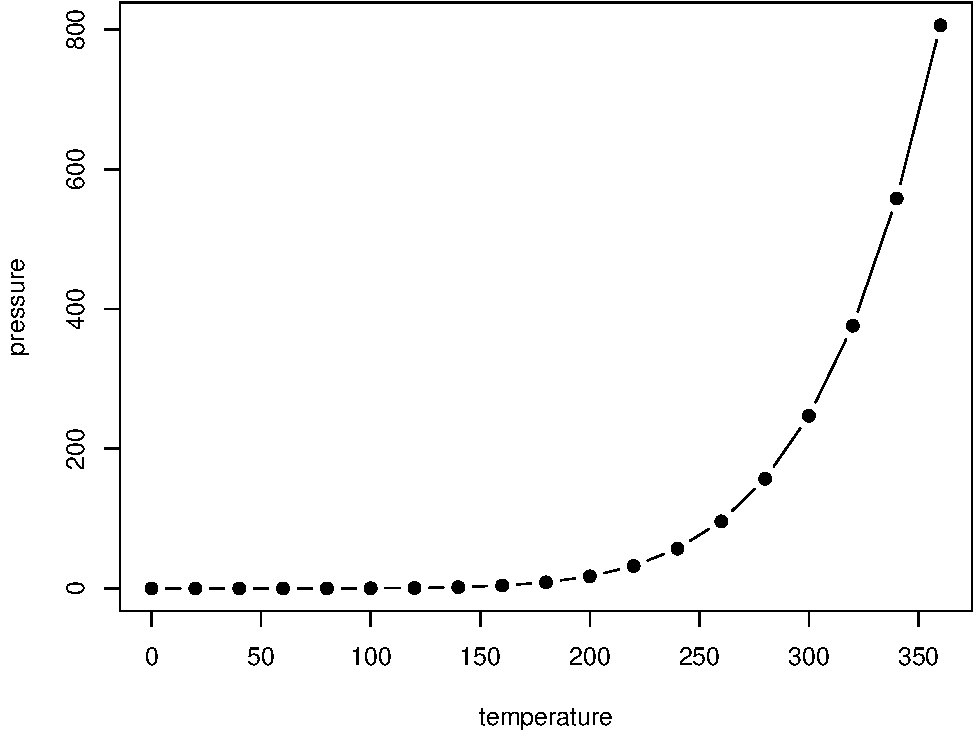
\includegraphics[width=0.8\linewidth]{scom-expb_files/figure-latex/fig01-01-1} 

}

\caption{En figur.}\label{fig:fig01-01}
\end{figure}

En linjär modell.

\begin{Shaded}
\begin{Highlighting}[]
\CommentTok{\# Predictor vs Criterion \{ggplot2\} {-} separate regression lines}
\NormalTok{gp =}\StringTok{ }\NormalTok{ggplot2}\OperatorTok{::}\KeywordTok{ggplot}\NormalTok{(}\DataTypeTok{data=}\NormalTok{iris, }
\NormalTok{ggplot2}\OperatorTok{::}\KeywordTok{aes}\NormalTok{(}\DataTypeTok{x=}\NormalTok{Sepal.Length,}
\DataTypeTok{y=}\NormalTok{Petal.Length,}
\DataTypeTok{colour=}\NormalTok{Species)) }\OperatorTok{+}\StringTok{ }
\NormalTok{ggplot2}\OperatorTok{::}\KeywordTok{geom\_smooth}\NormalTok{(}\DataTypeTok{method=}\NormalTok{lm) }\OperatorTok{+}\StringTok{ }
\NormalTok{ggplot2}\OperatorTok{::}\KeywordTok{geom\_point}\NormalTok{(}\DataTypeTok{size =} \DecValTok{2}\NormalTok{) }\OperatorTok{+}
\NormalTok{ggplot2}\OperatorTok{::}\KeywordTok{ggtitle}\NormalTok{(}\StringTok{"Sepal Length vs Petal Length"}\NormalTok{) }\OperatorTok{+}
\NormalTok{ggplot2}\OperatorTok{::}\KeywordTok{xlab}\NormalTok{(}\StringTok{"Sepal Length"}\NormalTok{) }\OperatorTok{+}\StringTok{ }\NormalTok{ggplot2}\OperatorTok{::}\KeywordTok{ylab}\NormalTok{(}\StringTok{"Petal Length"}\NormalTok{)}
\CommentTok{\#}
\KeywordTok{print}\NormalTok{(gp)}
\end{Highlighting}
\end{Shaded}

\begin{verbatim}
## `geom_smooth()` using formula 'y ~ x'
\end{verbatim}

\begin{figure}

{\centering 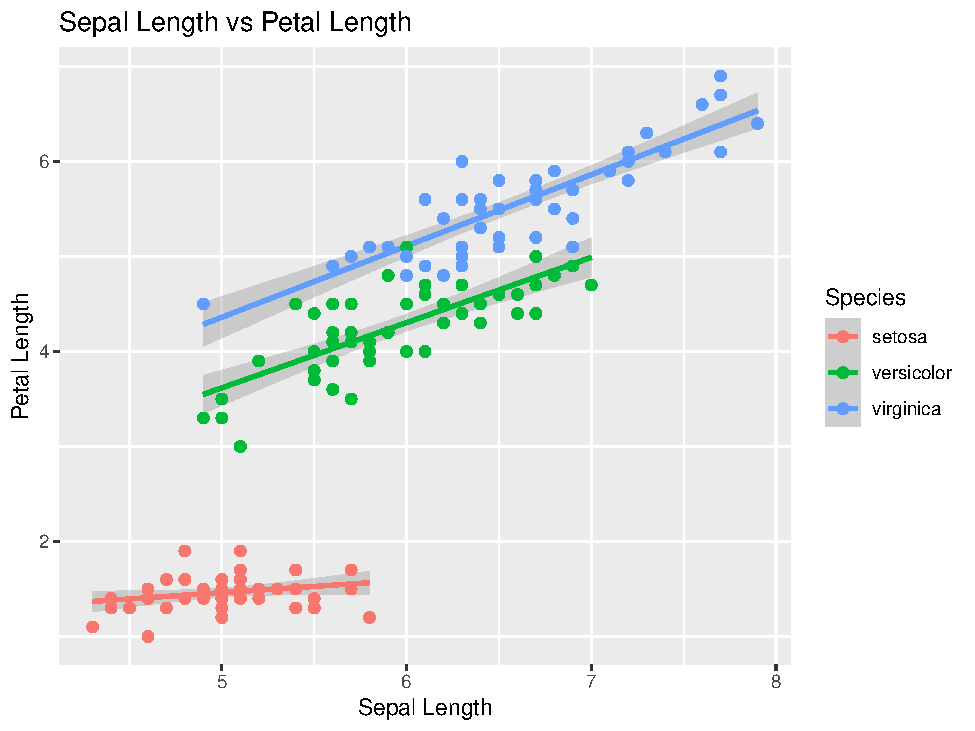
\includegraphics[width=0.8\linewidth]{scom-expb_files/figure-latex/fig01-02-1} 

}

\caption{Figur 1. Linjära modeller}\label{fig:fig01-02}
\end{figure}

\hypertarget{chap02}{%
\chapter{Kapitel}\label{chap02}}

I denna del av boken följer vi utvecklingen och genomförandet av ett samhällsvetenskapligt experiment. Exempel på en \textbf{tabell} kommer här:

\hypertarget{chap03}{%
\chapter{Kapitel}\label{chap03}}

I denna del av boken följer vi utvecklingen och genomförandet av ett samhällsvetenskapligt experiment. Exempel på en \textbf{referens} \citep{xie2015} kommer här.

\hypertarget{chap04}{%
\chapter{Kapitel}\label{chap04}}

I denna del av boken följer vi utvecklingen och genomförandet av ett samhällsvetenskapligt experiment.

\hypertarget{chap05}{%
\chapter{Kapitel}\label{chap05}}

I denna del av boken följer vi utvecklingen och genomförandet av ett samhällsvetenskapligt experiment.

\newpage

\hypertarget{part-del-2}{%
\part{Del 2}\label{part-del-2}}

\hypertarget{del-2}{%
\chapter*{Del 2}\label{del-2}}
\addcontentsline{toc}{chapter}{Del 2}

I denna del av boken följer vi utvecklingen och genomförandet av ett samhällsvetenskapligt experiment. Närmare bestämt kommer vi resonera kring ett tänkt experiment som tar avstamp inom kommunkationsforskningen, där man bland annat undersöker hur sociala medier såsom Facebook och Twitter används för att på olika sätt påverka mediepubliker. Till skillnad från den första delen av boken, där vi introducerade experiment som vetenskaplig metod, kommer del 2 att vara mer konkret och fokusera på de praktiska moment som ofta behöver beaktas i samband med planering, genomförande, och rapportering av ett experiment. Denna del av boken följer också ett kronologiskt upplägg, där vi börjar med att diskutera frågor som kommer tidigt i experiment-processen, och sedan övergår till att gå igenom praktiska frågor kring experimentets design. Vi kommer också använda oss av ett flertal andra konkreta experiment-exempel där detta krävs. Tanken med del 2 är att ge studenter ett ``matlagningsrecept'' för experimentella studier, där ``ingredienserna'' kan bytas ut och kombineras på nya sätt för att besvara nya frågeställningar. Vi är dock övertygade om att de flesta framgångsrika experiment följer vissa nödvändiga steg som successivt bygger på varandra. I denna bok kallat vi dessa steg för Förarbete (Kapitel 6), Genomförande (Kapitel 7), och Efterarbete (Kapitel 8).

\textbf{Förarbete.} I detta kapitel fokuserar vi på planeringsfasen i ett experiment. Denna fas är naturligtvis viktig oavsett vilken typ av studie vi ämnar genomföra, men på grund av att samhällsvetenskapliga experiment generellt sett vill undersöka hur en viss behandling påverkar människor, blir det avgörande att undersöka om och hur detta gjorts tidigare. Undersökningen av tidigare forskning tillåter oss att formulera (en eller flera) \emph{forskningsfrågor} som bygger vidare på tidigare forskningsresultat, och som därmed kan anses vara relevanta för forskningsfältet. När vi har formulerat forskningsfrågor med stöd av teoribildning och tidigare forskning har vi i nästa steg möjlighet att \emph{operationalisera} dessa frågor genom att omsätta kvalitativa begrepp till mätbara variabler. Detta steg kan vara så enkelt som att formulera en enkätfråga på ett sätt som visat sig vara framgångsrikt inom tidigare studier. När vi har operationaliserat forskningsfrågorna till mätbara variabler, kan vi åstadkomma den sista delen av förarbetet, i vilken vi formulerar \emph{hypoteser} om de statistiska samband vi förväntar oss att finna mellan våra mätvariabler. Allt detta förarbete till ett experiment är sådan information som ofta placeras i introduktionen till en uppsats eller forskningsartikel.

\textbf{Genomförande.} Detta kapitel behandlar de viktigaste praktiska stegen i experimentets genomförande. Dessa steg redovisas ofta utförligt i metoddelen av en uppsats eller forskningsartikel, och syftet med denna experimentbeskrivning är att möjliggöra upprepning av andra forskare. Genom att tidigt i forskningsprocessen göra ett \emph{pilottest} kan vi själva som forskare försäkra oss om att experimentet fungerar som vi har tänkt innan vi samlar in data. Därefter kommer den fullskaliga rekryteringen av \emph{försöksdeltagare} som nästa viktiga steg i genomförandet av ett experiment, och i detta steg är det viktigt att fundera på hur vi uppnår representativitet, samt hur vi rent praktiskt ska motivera personer att avsätta tid för att delta i studien och generera mätdata åt oss. När vi genomför ett experiment innebär det nästan alltid att vi använder någon form av \emph{mätinstrument} för att uppmäta hur våra försöksdeltagare svarar på en behandling. Denna behandling ingår i undersökningens \emph{experimentella villkor}, och tanken är ofta att konstrastera en uppmätt variabel mellan ett kontrollvillkor och ett behandlingsvillkor. Exakt hur varje deltagare genomgår dessa villkor definieras av den \emph{experimentella design} vi beslutat oss för att använda. När vi genomför experimentet är det viktigt att alla deltagare genomgår en standardiserad \emph{procedur} för att minska effekten av godtyckliga bruskällor i deltagarnas responser. Experimentets genomförande avslutas med \emph{dataanalys} som beskriver hur vi bearbetat mätvariablerna innan vi utvärderar effekten av våra experimentella villkor, vilket kommer att bli experimentents resultat.

\textbf{Efterarbete.} I detta kapitel tar vi upp: hur man kan redovisa resultatet av ett genomfört experiment, hur vi kan diskutera den samhälleliga och forskningsmässiga relevansen av undersökningen, samt hur resultaten kan rapporteras i form av en publicerad artikel. Naturligtvis förutsätter detta sista steg att vi klarat av de tidigare stegen. När vi är klara med själva genomförandet av ett experiment, brukar det första steget i efterarbetet vara att redovisa de \emph{resultat} undersökningen har lett fram till. Resultaten redovisas ofta i två steg, först med deskriptiva och sedan med inferentiella statistiska metoder. Den inferentiella statistiken används för att testa de hypoteser som inledningsvis uppställdes i förarbetet till experimentet, t.ex. att vi förväntade oss att hitta signifikanta skillnader mellan deltagarnas uppmätta responser i experimentets olika villkor. Efter att vi på detta sätt redovisat förhållandet mellan våra inledningsvis förväntade resultat och våra faktiska uppmätta resultat brukar man skriva en \emph{diskussion} om alternativa förklaringar till undersökningens observerade resultat, samt hur experimentet kan utvecklas och förbättras genom ytterligare forskning i framtiden. Avslutningsvis kommer detta kapitel diskutera vad forskare bör tänka på vid eventuell \emph{publicering} av forskningsresultat.

Genomgående försöker denna lärobok täcka in två olika men näraliggande betydelser av begreppet experimentell metod: dels som en uppsättning praktiska tillvägagångssätt som bör användas för att \emph{planera} och genomföra en experimentell studie; och dels som ett systematiskt och standardiserat sätt att i efterhand \emph{rapportera} genomförandet av en studie på ett sätt som är begripligt för andra forskare. Således är denna andra del av läroboken disponerat på ett sätt som ger oss möjlighet att i typisk turordning behandla de olika aspekter av experimentell metod som man som forskare förväntas kunna redovisa när man rapporterar sina resultat till en vetenskaplig tidskrift. Men inom varje metodaspekt kommer vi också att utförligt diskutera de olika experimentella tillvägagångssätt som är relevanta i samband med planering och genomförande av en forskningsstudie.

\hypertarget{chap06}{%
\chapter{Förarbete}\label{chap06}}

Innan man genomför ett experiment är det viktigt att noga undersöka om liknande experiment redan genomförts genom tidigare forskning. Inom samhällsvetenskapliga ämnen kan det exempelvis vara intressant att undersöka hur mediepublikers attityder, kunskaper och beteenden påverkas av olika typer av kommunikativa åtgärder (interventioner), t.ex. en marknadsföringskampanj eller ett politiskt budskap. På samma sätt är det inom medicinska vetenskaper ofta av intresse att utröna om ett nytt läkemedel har någon positiv effekt på patienter jämfört med en kur bestående av verkningslösa sockerpiller. Ju mer mån man är att undersöka ett tillförlitligt kausalt samband mellan en behandling och tillståndet hos målgrupp, desto viktigare blir det att kunna genomföra ett kontrollerat experiment, där effekterna av en behandling systematiskt jämförs med effekterna av en annan behandling (eller ingen behandling alls).

Det är inte ovanligt att en organisation som investerar pengar i en marknadsföringskampanj, också vill utvärdera olika kausala effekter av denna kommunikation på konsumenter. Genom att inventera tidigare forskningslitteratur inom detta specifika område, visar det sig ofta vilka mått och mätmetoder som använts, samt vad man kan förvänta sig om man genomför ett nytt experiment inom ett liknande experimentellt paradigm (REF). Framför allt kan tidigare forskning hjälpa oss att formulera några övergripande \emph{forskningsfrågor} som på något sätt för forskningsfältet framåt. Alla dessa aspekter av hur en ny, planerad studie förhåller sig till tidigare forskning, är viktiga genom hela forskningsprocessen. Tidigare använda mått och mätmetoder kan nämligen ge en god uppfattning om hur vi ska \emph{operationalisera} våra forskningsfrågor till mätbara variabler (mer om detta längre fram). Tidigare uppnådda resultat, å andra sidan, genererar vissa förväntningar om vilka resultat vårt eget experiment kommer att leda till, vilket i sin tur hjälper oss att formulera motiverade \emph{hypoteser} som är härledda från tidigare forskning inom området \citep{holmberg-2016-effects}.

Inom flera samhällsvetenskapliga discipliner har den konstruktivistiska kunskapssynen haft en framträdande roll under de senaste decennierna (ref). Som en konsekvens av detta har det blivit viktigt att ange en så kallad teoretisk referensram i samband med att man introducerar en kvalitativ forskningsstudie. Denna samling av teoretiska perspektiv (t.ex. retorisk eller semiotisk teoribildning) har sedan en viktig funktion vid analysen av empiriskt material, närmare bestämt genom att materialet tolkas med utgångspunkt i de teoretiska perspektiv man valt (därav den så kallade hermeneutiska forskningstraditionen). Inom den experimentella forskningen beskrivs kunskapssynen snarare som positivistisk, och teoretiska perspektiv används för att göra förutsägelser eller prediktioner om numeriska samband vi förväntar oss att hitta i kvantitiva mätdata. Detta gör att teorier generellt sett spelar en annan roll inom ett experiment jämfört med en kvalitativ studie, eftersom experiment använder empiriska resultat för att testa, och eventuellt uppdatera, befintlig teoribildning. Se även vetenskapsteori, Del 1.

När vi rapporterar förarbetet till ett experiment, görs detta ofta inom artikelns introduktion (jfr. akronymen IMRD i kapitel 8). När man introducerar en experimentell studie brukar man inleda med en kort bakgrund av det aktuella forskningsläget och en motivering till den genomförda undersökningen. Det är viktigt att det i ett tidigt skede står klart för läsaren vilket forskningsproblem (eller "kunskapsgap") studien vill bidra till att undersöka och helst råda bot på. Genomgången av tidigare forskning ska leda fram till och motivera den aktuella studiens forskningsfrågor och hypoteser. Det blir därmed viktigt att introduktionen och forskningsfrågorna refererar till empiriska resultat från tidigare forskning.

\hypertarget{sec06.1}{%
\section{Forskningsfrågor}\label{sec06.1}}

En viktig del av introduktionen till alla typer av vetenskapliga studier är att presentera studiens forskningsfrågor. Forskningsfrågor brukar i allmänhet vara nära kopplade till studiens syfte och mål, och bör därför vara möjliga att besvara inom ramen för studiens genomförande.

En forskningsfråga ska på ett någorlunda enkelt och kortfattat sätt sammanfatta vilka frågeställningar som ett specifikt experiment adresserar. Därför är det förhållandevis accepterat att forskningsfrågor är något abstrakt formulerade, så länge de ändå är enkla, lättfattliga och kortfattade. Introduktionens vidare uppgift är nämligen att konkretisera studiens forskningsfrågor genom en process som kallas \emph{operationalisering}, i vilken dessa forskningsfrågor omsätts till mätbara variabler som sedan kan ingå i falsifierbara \emph{hypoteser}. Man kan därför uttrycka det som att hypoteserna i en experimentell studie operationaliserar studiens forskningsfrågor. Operationalisering är ett mycket viktigt begrepp inom experimentell forskning, och vi återkommer mer utförligt till detta begrepp lite längre fram i detta kapitel, där vi också diskuterar hur detta begrepp hänger ihop med hypotesformulering.

\begin{table}

\caption{\label{tab:test-tab}This is a test table.}
\centering
\begin{tabular}[t]{lrr}
\toprule
col\_a & col\_b & col\_c\\
\midrule
a & 1 & 45\\
b & 2 & 46\\
c & 3 & 47\\
\bottomrule
\end{tabular}
\end{table}

Återgår vi till att diskutera begreppet forskningsfrågor mer generellt så finns det vissa tumregler som är viktiga att beakta. Den första tumregeln är att en forskningsfråga i någon del bör bygga på tidigare forskningsresultat, samt i någon del bör innehålla något nytt och outforskat. Med en sådan forskningsfråga kan man både upprepa (replikera) aspekter av tidigare forskning, men också utöka (extendera) tidigare forskning i syfte att skapa ny kunskap. En annan regel är att en forskningsfråga naturligtvis inte ska innehålla flera olika frågor, samt att två forskningsfrågor inte bör vara beroende av varandra (se övrig metodlitteratur, ref). Inom ramen för denna lärobok antar vi att en intressant forskningsfråga handlar om hur bildinnehållet i Facebook-poster påverkar läsarnas beteende och attityder. Närmare bestämt vill vi undersöka en upptäckt inom psykologisk forskning som visar att ett budskap upplevs som mer övertygande om det görs av en person som uppfattas som en auktoritet inom ett område (REF: Cialdini, 2001). Exempelvis kan vi föreslå att personen Leif GW Persson uppfattas som en auktoritet inom området kriminologi bland stora delar av den svenska mediepubliken. Vidare tänker vi oss att budskapet i en Facebook-post kan associeras med en auktoritetsperson genom att denna person visas i en bild som tillhör posten.

\hypertarget{sub06.1.1}{%
\subsection{Planering av forskningsfrågor}\label{sub06.1.1}}

I vårt tänkta experiment kretsar forskningsfrågorna kring effekterna av bildegenskaper hos Facebook-poster på internetanvändares visuella uppmärksamhet i samband med att de interagerar med dessa poster, samt effekter av bildinnehåll på användarnas självrapporterade nivå av upplevd trovärdighet hos samma poster. Låt oss anta att tidigare forskning ger vid handen att självskattad (eller upplevd) trovärdighet i nyhetsartiklar oftast har uppmätts med hjälp av enkätfrågor där försöksdeltagaren får besvara frågor av typen "Hur trovärdig var den nyhetsartikel du nyss läste?", genom att välja ett svarsalternativ på en 7-gradig skala, där värdet 1 innebär "Inte alls trovärdig", värdet 4 innebär "Varken trovärdig eller inte", samt värdet 7 betyder "Mycket trovärdig". Tidigare ögonrörelseforskning visar att pupillens position på en datorskärm är en bra indikator på vilka objekt på en webbsida som användaren riktar sin visuella uppmärksamhet mot. Detta samband är mycket användbart i föreliggande experiment, och kommer att diskuteras mer ingående nedan. Forskningsfrågor bör vara ganska generellt formulerade, vilket gör att de ofta kan ha ett nära samband med studiens målsättningar.

\hypertarget{sub06.1.2}{%
\subsection{Rapportering av forskningsfrågor}\label{sub06.1.2}}

När man arbetar med ett manuskript för en artikel eller uppsats så formuleras ofta forskningsfrågorna som "research questions", vilket ibland förkortas RQ. En studie kan naturligtvis fokusera på flera relaterade forskningsfrågor, men det vanligaste är att man adresserar en eller två huvudfrågor, som sedan kan delas in ytterligare i underfrågor (RQ1a, osv). Vissa vetenskapliga tidskrifter har en mycket strikt tolkning av experimentell metod, vilket innebär att hypoteserna i ett så kallat naturligt experiment bara kan kallas forskningsfrågor. Exempel på formulerade forskningsfrågor med anknytning till bokens exempel-experiment. Således, i vårt tänkta experiment skulle den första forskningsfrågan kunna formuleras:

\begin{itemize}
\tightlist
\item
  RQ1: Hur påverkar bildinnehållet i sociala medier-poster användarnas beteenden och attityder?
\end{itemize}

Som underfrågor till denna forskningsfråga skulle man kunna tänka sig "RQ1a: Hur påverkar bildinnehållet i Facebook-poster läsarnas blickbeteende", och "RQ1b: Hur påverkar bildinnehållet i Facebook-poster läsarnas attityder gällande postens trovärdighet".

\hypertarget{sec06.2}{%
\section{Operationalisering}\label{sec06.2}}

En annan mycket viktig del av förarbetet till ett experiment är att fundera på hur abstrakta begrepp inom forskningsfrågorna kan konkretiseras och omsätts till mätbara variabler. Denna process brukar kallas för \textbf{operationalisering}. För att utveckla detta resonemang kan det vara användbart med ett exempel. En samhällsvetenskaplig studie vill undersöka hur befolkningens attityder till miljövänlig sophantering har förändrats under senare år. Denna forskningsfråga innehåller som synes ett antal abstrakta begrepp (bl.a. "befolkning", "attityder", "miljövänlig" och "förändring") som behöver definieras och operationaliseras för att kunna studeras praktiskt. Ett sätt att operationalisera begreppet "attityder" i detta sammanhang vore kanske att intervjua ett antal personer om vad de tycker om miljövänlig sophantering. Detta kan potentiellt ge ett rikt och intressant empiriskt material i form av intervjusvar, men risken är att olika individer uppfattar denna fråga på olika sätt, vilket gör det svårt för forskarna att sammanställa resultaten av intervjun.

För att minska risken för subjektiva feltolkningar och förenkla sammanställningen av resultaten skulle forskarna kunna operationalisera begreppet "attityd" ytterligare genom att formulera påståenden av typen "det är viktigt att sophanteringen är miljövänlig", och därefter låter deltagaren svara på en 7-gradig skala, där värdet 1 betyder att man tar helt avstånd från påståendet, medan värdet 7 betyder att man helt instämmer. I detta fall omsätts attityd-begreppet till en variabel som kan anta värdena 1-7 (samt eventuellt värdet 0 om man väljer att inte svara). Standardisering, reliabilitet. Man kan också tänka sig att man försöker operationalisera attityder ytterligare genom att mäta kortisolnivåer i blodet. Kanske tänker man sig att starka attityder tar sig uttryck i en ökning av detta stresshormon? Även om detta skulle kunna genomföras som mycket objektiva och väldefinierade mätningar, så finns det förmodligen lite forskning som styrker ett samband mellan attityd och kortisolnivå, vilket gör detta till ett exempel på en dålig operationalisering som skulle resultera i en forskningsstudie med låg validitet eller giltighet.

I exemplet ovan har vi diskuterat olika operationaliseringar av medborgares attityder till en samhällsfråga. Den lägsta graden av operationalisering var att fråga ett antal undersökningsdeltagare vad de tycker i frågan och spela in intervjusvaren. Denna metod kräver omfattande efterbearbetning och kategorisering av materialet, och observationerna kommer att präglas av låg reliabilitet, då deltagares subjektiva tolkningar av attityd gör att svaren varierar på ett oförutsägbart sätt. En högre grad av operationalisering kan åstadkommas genom att istället låta deltagarna uttrycka sina attityder genom att ta ställning till hur lite eller mycket de instämmer i påståenden på en 7-gradig ordinalskala. Denna metod kräver mindre efterbearbetning för att sammanställa svaren, och eftersom både enkätfrågor och svarsalternativ presenteras i ett standardiserat format så ökar också reliabiliteten. Om vi analyserar tidigare forskning om attityder kommer vi också upptäcka att detta är ett beprövat sätt att operationalisera och undersöka just attityder, vilket indikerar att detta är en lämplig metod. Den högsta graden av operationalisering skulle kunna vara att mäta kortisolnivåer i blodet som en indikator på deltagarnas attityder. Även om detta skulle kunna ge oss mycket exakta, kontinuerliga, och tillförlitliga data på grund av att mätningarna är objektiva snarare än självrapporterade, så är detta ändå en olämplig metod eftersom den har en låg validitet eller giltighet i förhållande till fenomenet attityder.

Vad denna diskussion vill komma till är att operationalisering i grunden handlar om att omsätta ett kvalitativt begrepp till en kvantitativ mätvariabel, och detta är ett viktigt och nödvändigt moment i alla experimentella studier. Det finns ofta många sätt att operationalisera ett begrepp till en mätvariabel, men genom att konsultera tidigare forskning så får vi en fingervisning om mer och mindre lämpliga sätt att operationalisera. Begreppet operationalisering har också en koppling till distinktionen mellan olika datatyper och den varierande mängden information dessa datatyper anses innehålla. Lägre grad av operationalisering hänger då samman med mindre informationsmängd, t.ex. en kategorisk variabel (även kallat nominaldata). En datatyp med mer information och därmed högre operationalisering är ordinalskalor (eller likertskalor). Den högsta graden av operationalisering hänger samman med den mest informationsrika typen av data, eller kontinuerliga data (REF).

Från forskningsfråga till variabler. Våra forskningsfrågor handlar om hur egenskaper (s.k. faktorer) hos Facebook-poster påverkar läsares uppmärksamhet och upplevda trovärdighet. Baserat på tidigare psykologisk forskning tänker vi oss att bilder som innehåller auktoritetspersoner kan öka mängden visuell uppmärksamhet (beteende) på en Facebook-post samt öka upplevd trovärdighet (attityd) hos samma post. Givet detta sammanhang så blir mängden visuell uppmärksamhet, uppmätt som antal sekunder läsare tittar på Facebook-poster, vår första mätvariabel. Vidare blir upplevd trovärdighet, uppmätt på en skala från 1 (låg trovärdighet) till 7 (hög trovärdighet), vår andra mätvariabel. Dessa blir två mätvariabler kallas också för våra beroende variabler (mer om variabler i kapitel 7).

\hypertarget{sub06.2.1}{%
\subsection{Planering av operationalisering}\label{sub06.2.1}}

När vi väl etablerat vilka variabler som är våra beroende variabler, kan vi också definiera vilka variabler vi kommer använda för att förklara systematiska skillnader i mätvariablerna. Dessa kallar vi våra förklaringsvariabler, eller oberoende variabler. I vårt tänkta experiment kommer den viktigaste förklaringsvariabeln att utgöras av bildinnehållet i Facebook-poster, där innehållet kan variera mellan "auktoritetsperson" och "neutral person". Eftersom denna variation av bildinnehåll i grunden är en kvalitativ skillnad som inte på ett meningsfullt sätt kan kvantifieras, innebär det att förklaringsvariabeln är kategorisk snarare än en ordinalskala (som vi använder för att mäta deltagarnas attityder) eller en kontinuerlig skala (som används för att mäta hur länge deltagarna tittar på Facebook-posterna). I detta experiment förväntar vi oss alltså att variabeln "bildinnehåll" kommer att ha en kausal effekt på läsarnas blickbeteende och upplevelse av trovärdighet. En viktig del av operationalisering är att argumentera för att omsättningen av studiens begrepp till mätvariabler är giltig, dvs. präglas av validitet. Andra variabler som kan tänkas inverka på mätvariablerna i detta experiment är t.ex. demografiska variabler såsom ålder och kön hos deltagarna. Eftersom dessa variabler dock inte är centrala för vår frågeställning, kommer vi inte referera till dessa som oberoende variabler, utan som kontrollvariabler.

\hypertarget{sub06.2.2}{%
\subsection{Rapportering av operationalisering}\label{sub06.2.2}}

I vårt tänkta experiment kretsar forskningsfrågorna kring effekterna av bildegenskaper hos Facebook-poster på internetanvändares visuella uppmärksamhet i samband med att de interagerar med dessa poster, samt effekter av bildinnehåll på användarnas självrapporterade nivå av upplevd trovärdighet hos samma poster. Tidigare forskning ger vid handen att självskattad (eller upplevd) trovärdighet i nyhetsartiklar oftast har uppmätts med hjälp av enkätfrågor där försöksdeltagaren får besvara frågor av typen "Hur trovärdig var den nyhetsartikel du nyss läste?", genom att välja ett svarsalternativ på en 7-gradig skala, där värdet 1 innebär "Inte alls trovärdig", värdet 4 innebär "Varken trovärdig eller inte", samt värdet 7 betyder "Mycket trovärdig". Tidigare ögonrörelseforskning visar att pupillens position på en datorskärm är en bra indikator på vilka objekt på en webbsida som användaren riktar sin visuella uppmärksamhet mot. Därför är uppmätning av pupillposition på datorskärmen en lämplig operationalisering av visuell uppmärksamhet. Detta samband är mycket användbart i föreliggande experiment. Operationaliseringen av forskningsfrågorna rapporteras vanligen i introduktionen till en forskningsartikel.

\hypertarget{sec06.3}{%
\section{Hypotestestning}\label{sec06.3}}

Introduktionen av en forskningsartikel börjar alltså med att behandla studiens forskningsfrågor, dess centrala begrepp samt hur man gått tillväga för att operationalisera dessa begrepp i form av mätbara variabler. Efter att dessa aspekter har diskuterats är det lämpligt att introduktionen mynnar ut i studiens hypoteser. Den exakta formuleringen av dessa hypoteser är ofta ett av de mer krävande momenten i att genomföra en experimentell studie, eftersom hypoteserna löper som en röd tråd genom hela studien. Även om idealet är att hypoteserna ska formuleras tidigt i forskningsprocessen (studiens förarbete) och sedan inte förändras, så sker i praktiken ofta mindre justeringar av hypoteserna för att bättre anpassa dem till det faktiska genomförandet av studien.

Relationen mellan forskningsfrågor och hypoteser består i att om de förstnämnda uttrycks som generella frågor, så uttrycks hypoteser snarare som specifika och konkreta påståenden eller antaganden. Återgår vi till den forskningsfråga vi formulerade som exempel i denna lärobok, så löd den som följer: "RQ1: Hur påverkar bildinnehållet i Facebook-poster människors beteenden och attityder i relation till dessa poster?" Efter att vi formulerat denna forskningsfråga gick vi vidare till det moment vi kallar operationalisering, i vilket vi omsätter forskningsfrågan till mätbara variabler. I vårt fall utgick vi från tidigare forskning som visade att ögonrörelsemätning ofta använts för att objektivt observera och mäta människors visuella beteende i samband med att man läser texter på nätet. Vidare upptäckte vår forskningsgenomgång att människors attityder ofta undersökts genom självrapportering med hjälp av så kallade likert-skalor. I det sista steget använder vi de variabler som framkom i operationaliseringen till att formulera hypoteser. Närmare bestämt formuleras hypoteserna som förväntade relationer mellan förklaringsvariabeln "bildinnehåll" (dvs. auktoritetsperson eller neutral person) och mätvariablerna "visuell uppmärksamhet" och "upplevd trovärdighet". Sammanfattningsvis måste alltså hypoteserna vara underbyggda av tidigare forskning, och förväntade resultat måste motiveras utifrån tidigare erhållna forskningsresultat.

Det är inte ovanligt att en experimentell studie antar att det finns flera mätvariabler som påverkar en beroende variabl. I vårt exempel-experiment skulle vi till exempel kunna samla in mätdata om försöksdeltagarnas internetvanor och deras demografiska egenskaper, och undersöka hur dessa egenskaper bidrar till att förklara skillnader i exempelvis mängden visuell uppmärksamhet deltagarna spenderar på att titta på Facebook-posterna. I så fall antas hypoteserna gälla under en modell som inkluderar alla variabler. Detta kan visualiseras grafiskt med en modell.

\begin{figure}

{\centering 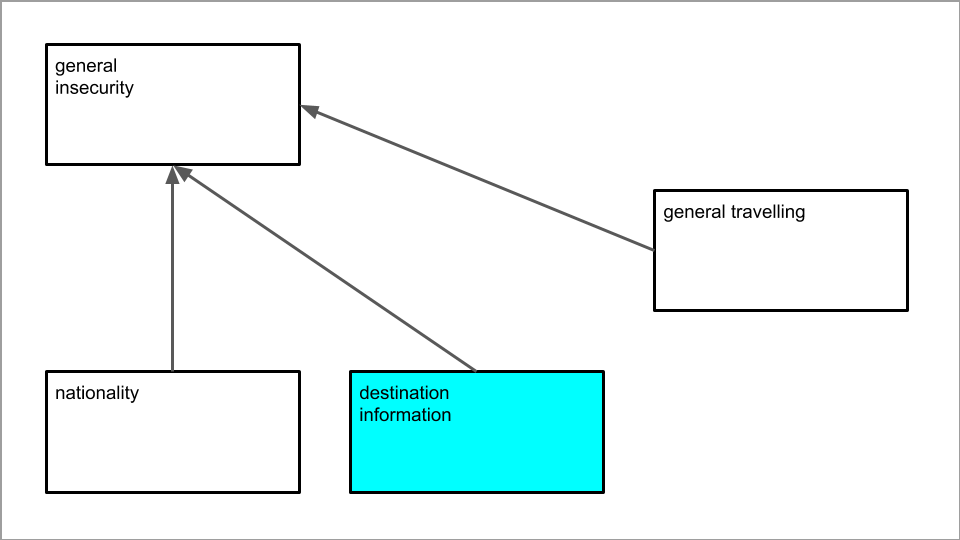
\includegraphics[width=0.8\linewidth]{../fig/model} 

}

\caption{en teoretisk modell}\label{fig:img-model}
\end{figure}

\hypertarget{sub06.3.1}{%
\subsection{Planering av hypoteser}\label{sub06.3.1}}

Inom flera samhällsvetenskapliga ämnen använder man sig av ett ramverk som kallas "Null Hypothesis Significance Testing" (förkortat NHST) i samband med att man formulerar hypoteser inom ett experiment (REF). Detta ramverk säger i princip att varje hypotes ska uttrycka endast \emph{ett} förväntat samband mellan studiens variabler. Hypoteserna ska vara formulerade så att \emph{riktningen} på förväntade samband framgår. I vårt experiment förväntar vi oss till exempel att när bildinnehållet varieras från "neutral person" till "auktoritetsperson" så kommer visuell uppmärksamhet och upplevd trovärdighet att öka. Vidare ska hypoteserna formuleras så att de går att falsifiera. Noll-hypotesen (H0) är att det inte finns någon statistiskt mätbar (signifikant) skillnad mellan villkoren. Om vi uppmäter en signifikant skillnad i våra beroende variabler mellan villkoren så förkastar vi noll-hypotesen. Det är mycket svårare att bevisa att ingen skillnad finns mellan två villkor, än att bevisa att en skillnad uppmätts (det förra alternativet kräver andra statistiska metoder som ibland kallas för Bayesianska).

\hypertarget{sub06.3.2}{%
\subsection{Rapportering av hypoteser}\label{sub06.3.2}}

Rapportering av hypoteser brukar komma i slutet av introduktionen, före rapportering av metoder. Till skillnad från generella forskningsfrågor, försöker vi formulera dessa hypoteser som specifika antaganden gällande samband mellan variabler. Styrkan med en experimentell studie är att vi kan formulera hypoteserna som kausala orsakssamband. När vi först manipulerar en oberoende förklaringsvariabel såsom "bildinnehåll" antar vi alltså att denna variation sedan \emph{orsakar} skillnader i de beroende variabler vi använder för att mäta försöksdeltagarna beteende och attityder. Inom vissa delar av den psykologiska forskningen kallas denna relation för stimulus-respons. Vi kan prata om kausala samband så länge det är ett kontrollerat experiment. Svårare om det är ett naturligt experiment. Slutligen ska riktningen på förväntade samband framgå. När vi tagit hänsyn till dessa kan vi sedan formulera en hypotes per beroende variabel som ingår i vår undersökning:

\begin{itemize}
\item
  H1: Facebook-poster med bild på en auktoritetsperson kommer att orsaka mer visuell uppmärksamhet på posten jämfört med bilder som innehåller en neutral person.
\item
  H2: Facebook-poster med bild på en auktoritetsperson kommer att orsaka högre upplevd trovärdighet hos posten jämfört med bilder som innehåller en neutral person.
\end{itemize}

Enligt NHST-modellen föregås dessa hypoteser egentligen av en så kallad noll-hypotes, under vilken vi antar att skillnader i bildinnehåll hos Facebook-poster \textbf{inte} kommer att orsaka några skillnader, varken vad gäller visuell uppmärksamhet eller upplevd trovärdighet. Noll-hypotesen brukar inte explicit skrivas ut då den är underförstådd, men den hade kunnat formuleras ungefär som: "H0: Facebook-poster med bild på en auktoritetsperson kommer inte att ha någon effekt på visuell uppmärksamhet (eller upplevd trovärdighet) gentemot posten jämfört med bilder som innehåller en neutral person". Detta innebär att om vår studie inte finner stöd för t.ex. den första hypotesen (H1) så är den falsifierad, och vi kan därmed antar att resultaten stödjer motsvarande noll-hypotes (H0).

The hypothetico-deductive model or method (step 1-4) this method can never absolutely verify (prove the truth of) 2. It can only falsify 2. This is what Einstein meant when he said, ``No amount of experimentation can ever prove me right; a single experiment can prove me wrong.'' \citep{einstein2002induction}

\hypertarget{sec06.4}{%
\section{Pre-registration}\label{sec06.4}}

TODO: Vad heter pre-registration på svenska? Kanske förregistrering. Koppling till open science framework: making research data and methods FAIR (findable, accessible, interoperable and reusable) and results reproducible. Här kommer en referens \citep{van2016pre} till denna relativt nya företeelse.

\hypertarget{chap07}{%
\chapter{Genomförande}\label{chap07}}

En av de viktigaste aspekterna av experimentell forskning handlar om att resultaten av ett specifikt experiment måste kunna reproduceras (eller replikeras) av en eller flera oberoende forskare. Om resultaten av ett experiment inte kan reproduceras, tyder detta på en godtycklighet i genomförandet, och man kan då med rätta ifrågasätta det forskningsmässiga värdet av ett sådan experiment. Om resultaten av ett experiment inte kan upprepas så kan de heller inte jämföras med tidigare eller efterföljande studier inom samma forskningsområde. Det blir alltså omöjligt att bygga vidare på icke-reproducerbara resultat, och de resurser i form av tid och pengar man spenderat på att genomföra studien kan till största delen betraktas som bortkastade.

För att ge utomstående forskare (och i högsta grad, oss själva) en möjlighet att upprepa en forskningsstudie och förhoppningsvis erhålla liknande resultat, krävs en utförlig och standardiserad dokumentation av hur studien genomförts (Berger, 1977). Denna dokumentation kallas för studiens metod. Metoddelen av en forskningsrapport ska alltså kunna fungera som tillräckligt detaljerade instruktioner för att andra forskare ska kunna återskapa alla de viktigaste betingelserna under vilka vi erhöll våra egna forskningsresultat, t.ex. antal deltagare, mätinstrument, dataanalys, osv (APA-standard). Men experimentell metod handlar naturligtvis också om att praktiskt tillämpa vissa tillvägagångssätt som utvecklats för att vi ska kunna försäkra oss om att genomförande och resultat är så giltiga och tillförlitliga som möjligt (se definitioner ovan).

I denna lärobok har vi försökt täcka in dessa två olika men näraliggande betydelser av begreppet experimentell metod: dels som ett systematiskt och standardiserat sätt att i efterhand \textbf{rapportera} genomförandet av en studie, och dels som en uppsättning praktiska tillvägagångssätt som bör användas för att i förväg \textbf{planera} och därefter genomföra en experimentell studie. Således är detta kapitel av läroboken disponerat på ett sätt som ger oss möjlighet att i typisk turordning behandla de olika aspekter av experimentell metod som man som forskare förväntas kunna redovisa när man rapporterar sina resultat till en vetenskaplig tidskrift. Men inom varje metodaspekt kommer vi också att utförligt diskutera de olika experimentella tillvägagångssätt som är relevanta i samband med planering och genomförande av en forskningsstudie.

I det följande kommer vi redogöra för den typiska turordningen för att både genomföra och rapportera ett experiment. Förarbetet är i detta skede redan avklarat, och genom att undersöka tidigare forskning har vi definierat en konceptuell forskningsfråga, som genom operationalisering omsatts till falsifierbara hypoteser.

\begin{itemize}
\item
  experimentell metod kan handla om att tänka baklänges, börja i hur resultaten rapporteras, och resonera sig fram till hur man ska planera studien
\item
  Ofta den första delen som skrivs när man rapporterar resultaten av en studie. Fördelaktigt att börja med en genomgång av hur studien faktiskt har genomförts.
\item
  kontrastera med metodologi, i del 1 ? Pedagogiskt att presentera efterföljande text som tre centrala beståndsdelar: 1) deltagare, 2) mätinstrument, och 3) experimentella villkor/manipulationer.
\end{itemize}

\hypertarget{sec07.1}{%
\section{Förstudier}\label{sec07.1}}

Innan man genomför ett skarpt experiment, vilket ofta kräver mycket resurser i form av tid och arbete, är det klokt att genomföra experimentet i liten skala. På så vis kan forskarna i ett tidigt stadium fånga upp problem med experimentdesignen. Detta kallas för att vi genomför en förstudie eller ett pilottest. I sambad med planering och förberedelse av experimentet kommer vi börja med att diskutera begreppet power-analys (från engelskans power analysis).

\hypertarget{sub07.1.1}{%
\subsection{Power-analys}\label{sub07.1.1}}

TODO: Innan man genomför ett skarpt experiment, gör en power-analys. Power is the probability that we will correctly reject the null hypothesis.

\begin{itemize}
\tightlist
\item
  Cohen, J. (1992)
\item
  Faul, F., Erdfelder, E., Lang, A. G., \& Buchner, A. (2007)
\item
  Faul, F., Erdfelder, E., Buchner, A., \& Lang, A. G. (2009)
\end{itemize}

\hypertarget{sub07.1.2}{%
\subsection{Pilottest}\label{sub07.1.2}}

Det är ofta användbart att förstå utvecklingen av en experimentell studie som en iterativ process, där genomförandet successivt kan förbättras baserat på erfarnheter från tidigare genomföranden. Slutligen är det ofta en fördel att kunna rapportera ett pilottest eller en förstudie i samband med att sakkunniga forskare granskar och bedömer om det är lämpligt att publicera resultaten i en tidskrift.

I pilottestet har vi möjlighet att testa att alla delar i experimentet fungerar, både som isolerade moduler oberoende av varandra, och som sammanhängande steg i en övergripande experimentell procedur. Vi kan alltså testa att vi kan rekrytera rätt \emph{försöksdeltagare}, dvs. deltagare som uppfyller de demografiska egenskaper som vi eventuellt specificerat i forskningsfrågor och hypoteser. Vi kan även testa att deltagarna förstår hur de lämnar informetat samtycke till att vi bearbetar den data vi samlar in från dem, samt andra etiska aspekter av vår forskning.

En annan del av experimentet som är mycket viktigt att testa och utvärdera har att göra med de \emph{mätinstrument} vi ämnar använda för att samla in data. Här kan det handla om att undersöka att deltagarna förstår enkätfrågorna i ett survey-experiment på det sätt som vi tänker oss att de ska förstå dessa frågor, och på det sätt som vi själva förstår dessa frågor. Det är inte ovanligt att vi som forskare får en helt annan förförståelse av enkätfrågorna i och med att vi formulerat dem, jämfört med hur en oinsatt försöksdeltagarna förstår frågorna. Lika viktigt är det naturligtvis att deltagarna förstår de responsalternativ som hänger samman med enkätfrågorna.

En annan sorts \emph{mätinstrument} utgörs av olika typer av sensorisk apparatur som kan användas för att samla in någon form av fysiologiska responser, exempelvis en ögonrörelsemätare (på engelska även kallad en eye-tracker) som används för att uppmäta var på datorskärmen deltagarna riktar sin visuella uppmärksamhet. Pilottest används i detta sammanhang för att försäkra oss om att vårt handhavande av mätutrustningen är korrekt (t.ex. kalibrering, applicering av elektroder på deltagaren o.dyl.), samt att datainsamligen genererar mätdata med tillfredställande nogrannhet (engelska accuracy, jfr. precision). Oavsett vilken typ av mätinstrument vi använder i ett experiment, är det alltså viktigt att noga överväga på instrumentents validitet och reliabilitet. Här kan tidigare forskning vara till stor hjälp, t.ex. genom framtagning av testade och validerade survey-frågor osv.

Nästa steg i förstudien handlar om att testa de behandlingar eller \emph{experimentella villkor} som vi planerar att administrera till våra försöksdeltagare. Genom att variera dessa villkor förväntar vi oss ju att kunna uppmäta skillnader i deltagarnas responser. Här underlättar det ofta att använda sig av termerna kontrollvillkor och behandlingsvillkor (ett eller flera). Exakt hur deltagarna exponeras för dessa villkor är en del av vår \emph{experimentella design}. Detta kan lösas genom att deltagarna exponeras för olika visuella stimuli som visas på en datorskärm. Ibland kan det krävas lite grundläggande programmeringskunskaper för att implementera en experimentell design (triggers etc.).

När vi har mätinstrument och experimentdesign på plats, kan det vara läge att pilottesta \emph{proceduren} vi kommer att använda oss av i samband med att varje deltagare genomgår vårt experiment. Denna procedur kan handla om allt från hur vi hälsar och tar emot deltagaren, till hur vi applicerar eventuell mätutrustning, till vi kort intervjuar deltagaren efter att den deltagit. Det främsta syftet med detta förfarande är att vi vill försäkra oss om att proceduren blir så standardiserad som möjligt, dvs. att vi inte eliciterar missvisande data från några deltagare pga. att dessa behandlats annorlunda i något avseende. I förlängningen har detta att göra med experimentets reliabilitet.

Slutligen är det väl värt att samla in lite faktisk testdata, när vi väl har alla experimentets delar på plats. Genom att göra detta kan vi pilottesta den \emph{dataanalys} som kommer ligga till grund för experimentets resultat. I denna fas testa vi helt enkelt att vi kan omvandla våra mätningar och villkor till variabler.

\hypertarget{sec07.2}{%
\section{Försöksdeltagare}\label{sec07.2}}

De individer som deltar i en studie kallades tidigare kort och gott "subjekt" (på engelska "subjects"). På senare tid har man vänt sig emot detta något avhumaniserande språkbruk och istället antagit den generella termen "deltagare". Här använder vi ibland beteckningen ``försökspersoner'' eller "försöksdeltagare" för att ytterligare betona den experimentella forskningens användning av kontrasterande behandlingar, villkor eller "försök" för att studera dess effekter på deltagarna (på engelska kallas sådana upprepade försök oftast för "trials", vilket är ett viktigt begrepp inom området experimentdesign som diskuteras längre fram i detta kapitel).

\hypertarget{sub07.2.1}{%
\subsection{Representativt urval}\label{sub07.2.1}}

Inom samhällsvetenskapliga forskningsområden är det vanligt att anta att deltagarna i en studie ska vara så representativa som möjligt i förhållande till en viss målpopulation. Tanken bakom detta är att man av praktiska skäl bara har möjlighet att inkludera en mindre grupp deltagare i en studie (t.ex. studenter på ett visst utbildningsprogram), och utifrån detta begränsade urval vill man sedan kunna generalisera undersökningens resultat till en större grupp människor (t.ex. alla universitetsstuderande i Sverige). Även om detta resonemang i grund och botten är rimligt, är det främst användbart inom större enkätstudier som syftar till att undersöka attityder, kunskaper och beteenden hos en avgränsad och väldefinierad population av individer. Ett annat vanligt exempel på enkätundersökning där deltagarnas representativitet är avgörande är politiska opinionsundersökningar. Utifrån drygt tusen deltagare vill man här kunna generalisera till hela Sveriges befolkning med relativt låg felmarginal.

- ska vi ta upp termer som ``obundet slumpmässig urval'', stratifierat urval, bekvämlighetsurval, snöbollsurval (inom intervjustudier)?

\hypertarget{sub07.2.2}{%
\subsection{Demografiska egenskaper}\label{sub07.2.2}}

Inom experimentell forskning tenderar man att tänka lite annorlunda kring frågan om att erhålla ett representativt urval av försöksdeltagare till en studie. Det är framför allt två saker som föranleder detta. För det första är det vanligt att man använder sig av objektiva och mätbara observationer i ett experiment, till skillnad från subjektiva (självrapporterade) och kvalitativa observationer i en survey, vilket antas leda till lägre nivåer av brus i de mätningar som genomförs. För det andra är det vanligt att de experimentella effekter man studerar är så små och svåra att uppmäta, att alltför stora individuella skillnader hos deltagarna riskerar att generera så mycket brus att effekten av en behandling inte kan detekteras. Av dessa två skäl är det vanligt att man eftersträvar någorlunda homogena deltagargrupper när man syftar till att genomföra experimentella studier.

Att man delvis frångår principen om representativt urval inom experimentell metodik har alltså att göra med att man på olika sätt vill begränsa mängden slumpartade och systematiska mätfel, dvs brus. Detta är ett tänk som kommer från det naturvetenskapliga området signalbehandling (ref). Nackdelen med detta förfarande är naturligtvis att generaliserbarheten riskerar att minska, vilket oftast är en svaghet. Inom vissa utbildningssystem där deltagande i experimentella studier är obligatoriskt för studenter, har den experimentella forskningen kritiserats för att endast kunna generalisera till just den befolkningsgrupp som studenter vanligtvis tillhör, t.ex. 18-25-åringar med västerländskt ursprung och förhållandevis god socioekonomisk ställning (ref). Referera till begreppen bakgrundsvariabler, kontrollvariabler.

En annan faktor som har stor betydelse i samband med urvalet av försöksdeltagare är naturligtvis om de forskningsfrågor man undersöker är kopplade till någon specifik befolkningsgrupp, t.ex. vad gäller ålder (barn eller äldre), språk (enspråkiga eller flerspråkiga) och kognition (funktionsnedsatta och normalbefolkning). Om så är fallet, blir det ju naturligt att rekrytera deltagare från just dessa grupper och därmed ge avkall på möjligheten att kunna generalisera sina resultat till en bredare population. I viss mån styrs alltså urvalet av försöksdeltagare av den tidigare forskning som vi med vårt experiment vill bygga vidare på och kontribuera till. Som en tumregel kan man dock säga att en experimentell studie brukar bygga på 20-100 deltagare, där åldersspannet inte är för stort, och könsfördelningen inte är för skev. Längre fram i detta kapitel kommer vi även att diskutera hur experimentdesign påverkar antalet deltagare som är lämpligt i en studie.

\hypertarget{sub07.2.3}{%
\subsection{Etiska hänsynstaganden}\label{sub07.2.3}}

En internationell trend inom samhällsvetenskaplig forskning som gjort sig gällande under senare år är att stor vikt läggs vid forskarens etiska hänsyn gentemot dess försöksdeltagare. Exempelvis kan en journal kräva att ett experiment genomgått en etisk prövning innan det genomförs, i annat fall vill tidskriften inte publicera resultaten. Detta är naturligtvis i grunden en positiv utveckling, men det adderar ofta ett administrativt moment som behöver klaras av innan en studie kan sättas i verket. När en etisk kommitté utvärderar ett experiment är det framför allt två aspekter man tar hänsyn till: 1) att deltagaren inte ska lida några men i samband med genomförandet av undersökningen, och 2) att forskaren har en genomtänkt plan för hantering av forskningsdata som samlas in. Ett exempel på den första aspekten är analysera vilka villkor och manipulationer som förekommer, samt om mätutrustningen är invasiv eller inte. Exempel på det andra hänsynstagandet är att försöksdeltagares personliga integritet inte ska bli lidande (t.ex. känsliga personuppgifter), samt att forskningsdata ska hanteras på ett säkert sätt som även tillåter deltagaren att begära ut sina uppgifter i efterhand. Som regel är dessa hänsyn viktigare för anställda forskare; för studentprojekt brukar inte etisk prövning av studier vara nödvändigt.

\hypertarget{sub07.2.4}{%
\subsection{Planering av deltagare}\label{sub07.2.4}}

Här kommer några praktiska råd i samband med att man rekryterar försöksdeltagare till en experimentell studie. För det första, underskatta inte betydelsen av att få tillgång till motiverade personer som dels är omedvetna om syftet med experimentet, och dels är någorlunda representativa för den grupp av människor resultaten ska kunna generaliseras till. För det andra, underskatta inte den tid och möda som krävs för att lösa de logistiska aspekterna av att låta ett hundratal(?) individer genomgå de behandlingar som ett experiment består av under kontrollerade och likartade förutsättningar. Både bland forskare och studenter finns en föreställning om att planering av försöksdeltagare löser sig självt; så är dock inte fallet.

Redan på ett tidigt stadium är det viktigt att fastställa om det planerade experimentet är av en sådan art att det kräver etisk prövning, och i så fall måste studien godkännas av en etisk nämnd innan rekrytering av deltagare påbörjas. Etisk prövning blir ofta aktuellt om känsliga personuppgifter eller biometriska data samlas in, och om invasiv försöksutrustning som på något sätt kan förväntas påverka deltagaren används. I vårt exempel-experiment uppfylls inte dessa kriterier, eftersom tanken är att manipulera bildinnehåll i Facebook-poster, samt samla in data om deltagarnas blickbeteende och attityder.

Förutsatt att inga etiska hinder föreligger, kan rekryteringen av försöksdeltagare påbörjas genom att förslagsvis annonsera om studien och förse intresserade personer med kontaktuppgifter till försöksledaren (epost, telefonnummer, webblänk), samt möjlighet för presumtiva deltagare att ange dag och tid när de har möjlighet att delta. För att öka chanserna att folk ska anmäla sig till undersökningen kan det vara fördelaktigt att erbjuda någon form av ersättning, t.ex. en biobiljett eller en lunchkupong, dock underlättar det om ersättningsnivån inte överstiga ca 100 kr eftersom det då blir beskattningsbar inkomst.

I praktiken är det dock kanske viktigare att prata med tilltänkta försöksdeltagare och göra dem intresserade av forskningen och motiverade att avsätta tid för deltagande. Denna information måste då vägas mot att deltagarna ska vara omedvetna om syftet med det tilltänkta experimentet. Utgår vi återigen från vårt exempel-experiment, innebär detta att vi kan informera om att studien undersöker Facebook-användning, men att vi undanhåller hur vi manipulerat bildinnehållet i Facebookposterna (auktoritetspersoner gentemot neutrala personer). På forskningsjargong innebär detta att deltagarna avsiktligt hålls omedvetna eller "naiva" om studiens behandlingar, och att detta i sin tur minskar risken för påverkan eller "bias" i de observationer som samlas in.

Om vi förflyttar oss framåt i tiden till själva genomförandet av studien, så är det viktigt att betänka att varje försöksdeltagare ska ha rätt att ge informerat samtycke till studien innan den deltar (den engelska termen för detta är "informed consent"). Om deltagaren är yngre än 15 år krävs \textbf{dessutom} alla vårdnadshavares samtycke. Detta innebär att försöksledarna i förväg har en informationssida som beskriver forskarens respektive deltagarens rätt- och skyldigheter. Detta dokument ska undertecknas av deltagaren innan experimentet påbörjas.

Forskaren har rätt att: använda insamlade data för publikationer

Forskaren är skyldig att: beskriva mätutrustning, t.ex. att en ögonrörelsemätare kommer mäta pupillens position i relation till datorskärmen.. beskriva vilka data som samlas in och generellt syfte.. förvara data säkert

Deltagaren har rätt att: få sina data utlämnade (raderade om ingen anonymisering)

Deltagaren är skyldig att: Signera att ersättning tagits emot

\hypertarget{sub07.2.5}{%
\subsection{Rapportering av deltagare}\label{sub07.2.5}}

När man väl genomfört studien och är i färd med att rapportera vilka personer som deltagit så krävs det vanligtvis betydligt mindre arbete än i planerings- och genomförandefasen. I artikeltexten läggs information om experimentets försöksdeltagare ofta som den första underrubriken till metodstycket, och det är också därför vi tar upp försöksdeltagare på just detta ställe i läroboken. Anledningen till att vi använder denna så kallade IMRD-disposition är det skapar en kronologisk struktur för både planering och rapportering av vetenskapliga studier, och för de som vill genomföra ett experiment kan det vara värdefullt att bekanta sig med denna konvention.

- demografiska variabler, medelålder, range

- exempel på hur detta skulle kunna formuleras i ett manuskript, på engelska?

- representativt urval, population, bakgrundsvariabler, individuell variation

- bortfall, missing cases

\hypertarget{sec07.3}{%
\section{Mätinstrument}\label{sec07.3}}

I en experimentell studie är det avgörande att införliva mätinstrument som på ett giltigt och tillförlitligt sätt kan uppmäta effekten av en behandling på en eller flera responsvariabler. En viktig anledning till att experiment och mätinstrument är nära förknippade, är att denna typ av positivistisk forskning syftar till att försöka säkerställa en faktisk skillnad mellan olika grupper av deltagare och olika typer av behandlingar, vilket till syvende och sist kräver analys med hjälp av statistiska metoder. Det räcker alltså inte med att forskaren rapporterar en subjektivt upplevd skillnad mellan försöksgrupper; denna skillnad måste bevisas!

I detta sammanhang bör mätinstrument uppfattas som ett relativt abstrakt begrepp; det kan röra sig om medicinsk eller fysiologisk mätutrustning, men i många samhällsvetenskapliga ämnen handlar mätinstrument ofta om enkätfrågor där svarsalternativen är utformade som Likert-skalor, exempelvis med skalsteg från 1-7. Med hjälp av ett sådant survey-instrument tänker man sig att det går att uppmäta försöksdeltagarnas attityder kring något ämne. Men man skulle också kunna tänka sig ett experiment inom marknadsföring som använder en binär mätvariabel. I detta fall skulle två deltagargrupper kanske titta på varsin version av en reklamfilm, och sedan svara "ja" eller "nej" på frågan om de var intresserade av att köpa den produkt som marknadsfördes i båda filmerna.

I det hypotetiska experiment som vi resonerar om i denna bok används två olika mätinstrument för att registrera olika typer av responser hos deltagarna i samband med att de tittar på Facebook-poster med bilder föreställande auktoritetspersoner respektive neutrala eller okända personer. I första steget används en ögonrörelsemätare för att mäta hur försöksdeltagarna visuella uppmärksamhet fördelar sig över Facebook-posten, och sedan används en 7-gradig Likert-skala för att mäta hur bildinnehållet påverkat deras attityder angående postens trovärdighet. De hypoteser som antagits för detta experiment är att auktoritetspersoner kommer att orsaka en ökning av visuell uppmärksamhet (dvs. hur länge deltagarna tittar på bilden), samt en ökning av upplevd trovärdighet hos posten (dvs. hur höga värden som väljs på Likert-skalan). En viktig skillnad mellan dessa två mätinstrument är att ögonrörelsemätning fångar ett objektivt beteende hos deltagaren, medan Likert-skalor registrerar mer subjektiva responser som rapporteras av deltagaren själv. Denna skillnad utvecklas lite mer i det följande (avsnitt \protect\hyperlink{sub07.3.2}{7.3.2}).

\hypertarget{sub07.3.1}{%
\subsection{Olika mätnivåer}\label{sub07.3.1}}

TODO: Ta upp levels of measurement. Olika mätnivåer. Nominal, Kvot-skala. Intervall. Nominal tillåter bara analyser som handlar om att räkna antal förekomster. Ta upp psychopy3 2020 som exempel.

\hypertarget{sub07.3.2}{%
\subsection{Mätning av subjektiva responser}\label{sub07.3.2}}

En subjektiv respons innebär att det är helt upp till försöksdeltagaren att avgöra vilka mätdata man vill och kan lämna. Denna situation uppstår med nödvändighet i alla former av enkätfrågor, där själva frågekonstruktionen är öppen för deltagarens tolkning, och där deltagaren själv får bestämma vilket svarsalternativ den väljer att lämna som respons. Dessutom kan det uppstå systematiska felkällor (s.k. bias) beroende på hur forskaren samlar in svaren (t.ex. genom intervju eller skriftligt). Det är lätt att inse att ett sådant mätinstrument gör sig beroende av varje deltagares individuella förmåga och motivation att lämna giltiga svar, och att den mätdata som samlas in kommer att innehålla olika former av bruskällor som kan förvränga de sanna mätvärdena.

Även om enkätfrågor därmed kanske inte kan betraktas som en perfekt lösning, används de ändå flitigt inom den samhällsvetenskapliga forskningen, av det enkla skälet att detta mätinstrument ofta är det enda realistiska alternativet som står till buds om vi exempelvis avser att mäta deltagarnas attityder till ett fenomen, eller andra typer av mentala tillstånd. Man brukar säga att enkäter är lämpliga för att mäta deltagarnas \emph{beteenden} (t.ex. hur ofta de använder sociala medier på ett dygn), \emph{kunskaper} (t.ex. hur mycket de känner till om de algoritmer sociala medier använder för att presentera personligt innehåll till användaren), och \emph{attityder} (t.ex. om de har förtoende för hur sociala medier hanterar användarens personliga data).

För att hantera några av enkätens inneboende problem som mätinstrument har forskningen både förfinat själva frågedelen i enkäten, men också svarsalternativen. Detta kan åskådliggöras genom ett resonemang där vi antar att vi som forskare är intresserade av att mäta upplevd lycka bland en grupp människor. I detta exempel säger vi att det mentala tillståndet lycka är en latent variabel som vi inte kan mäta direkt, men som vi försöker komma åt genom att använda ett antal enkätfrågor som antas fånga olika aspekter av konceptet lycka. En fråga kan lyda ``hur lycklig är du i hemmet?'', en annan ``hur lycklig är du på jobbet?'', en tredje ``hur lycklig är du med dina vänner?'' osv. Förhoppningen är att flera likartade frågor sammantaget ska öka giltigheten (validiteten) i mätinstrumentet.

När det gäller svarsalternativ till dessa tänkta enkätfrågor om lycka, är det vanligt att använda så kallade likert-skalor, där deltagaren kan indikera ett värde mellan exempelvis 1 och 7, där lägre och högre värden betyder mindre respektive mer upplevd lycka, och mittenalternativet är neutralt. Genom att använda likartade skalor på flera enkätfrågor skapas ett någorlunda standardiserat format för svarsalternativen som deltagaren förhoppningsvis har lättare att ta ställning till. De numeriska värden som erhålls på varje individuell fråga kan sedan sammaställas till ett så kallat index genom att ta medelvärdet av deltagarens alla responser kring lycka. Detta antas öka tillförlitligheten eller reliabiliteten i mätinstrumentet. Men kom ihåg att denna typ av data är självrapporterad!

\hypertarget{sub07.3.3}{%
\subsection{Mätning av objektiva responser}\label{sub07.3.3}}

Objektiva responser är inte väsenskilda från subjektiva, och därför är det mer fruktbart att placera båda dessa responser på en skala av objektivitet, där enkätfrågor kan betraktas som mindre objektiva, och exempelvis fysiologiska responser anses mer objektiva. När det gäller enkätfrågor så betraktas ibland frågor som avser att undersöka respondentens beteenden som mer objektiva än frågor som frågor handlar om attityder (ref). Om vi flyttar fokus till fysiologiska mätmetoder så kan vi på samma sätt skilja mellan responser som är mer viljestyrda hos deltagaren (t.ex. var blicken riktas på en datorskärm), respektive mätdata som är mindre viljestyrd (t.ex. hur utvidgade pupillerna är). Det förra fallet handlar om mindre objektiva responser, det senare om mer objektiva. Subjektiva och objektiva responser är alltså ingen absolut distinktion.

\begin{table}

\caption{\label{tab:tab02-07-3}Mätinstrument och objektivitet i mätdata}
\centering
\begin{tabular}[t]{llll}
\toprule
minst objektiv & mindre objektiv & mer objektiv & mest objektiv\\
\midrule
attitydfrågor & beteendefrågor & voluntär respons & involuntär respons\\
\bottomrule
\end{tabular}
\end{table}

Låt oss utveckla resonemanget kring fysiologisk mätdata som potentiellt mer objektiva responser. Inom psykologisk, beteendevetenskaplig och medicinsk forskning skiljer man ofta på fysiska responser som är voluntära (viljestyrda) respektive involunära (icke-viljestyrda). Detta kan exemplifieras genom att betänka människans synsystem, där vi ibland viljemässigt styr vår visuella uppmärksamhet mot en specifik region i synfältet (endogenous attention), men ibland riktar blicken som en reflexmässig respons på att något oväntat plötsligt händer i vår omgivning (exogenous attention). Dessutom kan vi ibland rikta vår visuella uppmärksamhet mot något utan att direkt titta på det.

Detta resonemang säger oss att pupillens position \emph{ofta} utgör en relativt exakt indikator på var försöksdeltagaren riktar sin visuella uppmärksamhet, även om det finns undantag. Detta samband gör att vi kan använda ögonrörelsemätning som en mätmetod med hög grad av objektivitet och giltighet i situationer där vi vill förstå vilka yttre orsaker som påverkar visuell uppmärksamhet. I dessa situationer utgör visuell uppmärksamhet en latent variabel kopplad till människans kognition. Vi är ofta intresserade av att uttala om sådana kognitiva processer, men vi kan sällan direkt observera dem. Därför använder vi oss i detta fall av ögonrörelsemätning som en objektiv indikator på visuell uppmärksamhet.

För att ögonrörelsmätning ska fungera som en objektiv indikator för visuell uppmärksamhet krävs också att vi kan samla in data utan systematiska avvikelser (s.k. bias). Systematiska avvikelser kan inträffa om vi ställer in mätinstrumentet på ett felaktigt sätt, vilket exempelvis skulle kunna resultera i att alla uppmätta pupillpositioner förskjuts i någon rikting, vilket i sin tur betyder att vi relaterar deltagarens visuella uppmärksamhet till fel objekt på datorskärmen. För att undvika detta krävs kunskap om hur mätinstrumentet bör handhas, samt om hur vi kan kaliberera systemet för att ge tillförlitlig data oberoende av deltagarnas individuella fysiska egenskaper.

Andra exempel på fysiologiska och beteendevetenskapliga mätdata kan utgöras av observationer kopplade till deltagares användning av en webbläsare för att navigera en webbplats, t.ex. hur de använder en sökfunktion, hur länge de tittar på en video, eller vilka länkar de väljer att klicka på. Reaktionstidstest är också ganska vanligt. I dessa fall kan det vara underliggande kognitiva beslutprocesser som är av intresse för forskarna, eller så kan det vara klick-data i sig som är intressant. I många fall av fysiologisk datainsamling blir det viktigt att instruera deltagarna att genomföra någon form av uppgift i samband med att data spelas in. Detta för att minska variationen mellan individier (osystematiskt brus i data). Detta kan kräva mycket planering i studiens tillvägagångssätt. Instruktionen i vårt tänkta experiment skulle antagligen bli något i stil med ``försök bedömma trovärdigheten i följande fb-poster''. Detta för öka validitet och reliabilitet.

Här kan vi eventuellt använda en analogi från rättsväsendet, där man ibland skiljer mellan indicier (t.ex. vittnesuppgifter) och fysiskt bindande bevisning. Indicier handlar om bevismaterial som är mer subjektiva och därmed föremål för tolkning, vilket gör att det krävs mer sådan. Medicinska experiment där vi objektivt mäter 1) aktiv substans, 2) egenskaper hos deltagare, 3) antal viruspartiklar i blodet. Denna typ av direkta mätningar är inte alltid relevant inom samhällsvetenskaplig forskning.

\hypertarget{sub07.3.4}{%
\subsection{Beroende variabler}\label{sub07.3.4}}

I det tänkta experiment som ligger till grund för denna bok, använder vi oss huvudsakligen av två mätinstrument. Vi använder en så kallad ögonrörelsemätare (på engelska "eye-tracker") för att göra objektiva och kontinuerliga mätningar av hur läsarnas visuella uppmärksamhet fördelar sig över ytan på de Facebook-artiklar vi visar som stimuli på en datorskärm. Därefter använder vi en digital enkät som presenteras på samma datorskärmen \emph{efter} varje Facebook-post. Enkäten består av två-tre frågor om hur försöksdeltagaren upplever trovärdigheten i varje Facebook-post, och varje enkätfråga är kopplad till en likert-skala, där och olika aspekter av upplevd trovärdighet mäts på en skala mellan 1 och 7, och där högre värden används för att indikera högre trovärdighet.

Här gäller det att hålla i minnet att hälften av Facebook-posterna vi använder som stimuli i vår studie innehåller en bild på en okänd och därmed neutral person. Dessa stimuli används som experimentets kontrollvillkor. Den andra hälften av Facebookposterna kontrasterar mot detta villkor genom att innehålla bilder på auktoritetspersoner. Vi säger därmed att den senare hälften av posterna innehåller en behandling eller manipulation, vilket gör att dessa stimuli representerar det experimentets behandlingsvillkor. Vägledda av tidigare forskning inom denna medie- och kommunikationsforskning förväntar vi oss att stimuli som innehåller manipulationen ``bild på auktoritetsperson'' ska medföra en effekt på deltagarnas uppmätta responser. Eftersom vi tänker oss att responserna på ett systematiskt sätt \emph{beror} på en föregående behandling, kallar vi dessa responser för beroende variabler. Ibland kallas de också för utfallsvariabler eller responsvariabler.

Syftar generellt till att uppmäta och registrera en respons på ett stimuli eller en behandling, därför säger man ibland att syftet med mätinstrumenten är att på ett giltigt och tillförlitligt sätt mäta en responsvariabel. Ofta kontinuerlig eller binär (logistisk regression), men kan också vara multinomial eller kategorisk. Survey-frågor, svarsalternativ, likertskalor, attityder. "Beror" av en kronologiskt föregående orsak, dvs. behandling. På engelska kallas detta "dependent variable". Beroende variabler kallas ibland också mätvariabler eller utfallsvariabler. Jämför med oberoende variabler, förklaringsvariabler, experimentella villkor, behandlingar i nästa stycke av boken. På engelska "independent variable". Varje modell har \emph{en} beroende, flera oberoende variabler. Kausala samband har potentiellt större förklaringsvärde än associativa samband (korrelationer).

\hypertarget{sub07.3.5}{%
\subsection{Planering av mätinstrument}\label{sub07.3.5}}

När vi genomför ett experiment kräver detta nogrann planering av de mätinstrument vi avser att använda för att uppmäta deltagarnas responser i relation till kontrollvillkor respektive behandling. Ett typiskt experiment omfattar oftast mätning av \emph{en} responsvariabel, men i det tänkta experiment vi diskuterar i denna bok, mäter vi \emph{två} typer av responser med olika mätinstrument. Förutom att vi behöver planera hur vi ska använda varje enskilt mätinstrument, behöver vi alltså också planera för hur vi ska kombinera dessa mätningar. Den viktigaste principen här är att designa experimentet så att den ena mätningen inte alltför mycket påverkar den andra mätningen (systematiskt bias). Som exempel kan vi tänka oss en situation där vi först använder en survey för att mäta deltagarnas generella tilltro till innehåll på sociala medier, och sedan mäter deltagarnas visuella uppmärksamhet på en Facebook-post. I denna situation får vi anta den första mätningen (survey) till viss del influerar eller ``spiller över'' på den andra mätningen (blickbeteende). Beroende på vilken frågeställning experimentet är tänkt att svara på, kan detta vara mer eller mindre problematiskt. Generellt kan man säga att denna typ av priming-effekter bör minimeras, men ibland är de oundvikliga, och ibland är de till och med önskvärda (t.ex. i priming-experiment).

I denna bok använder vi ögonrörelsemätning som ett slags representant för flera typer av mätmetoder som kan kallas beteendevetenskapliga eller fysiologiska, dvs att de ämnar mäta npgon form av fysiska responser och/eller viljestyrt beteende. Förutom ögonrörelsemätning, är det ganska vanligt att man mäter hjärnaktivitet med hjälp av apparatur som kallas elektroencefalografi (EEG) eller magnetresonansavbildning (fMRI), eller reaktionstider uppmätt med hjälp av tagenttryckningar, eller datorinteraktion uppmätt med hjälp av datormus och tangentbord. I fallet med ögonrörelsemätning, liksom övriga nyss nämnda fysiologiska mätmetoder, är det vanligt att experimentledaren behöver en separat utbildning i hur systemet ska användas för att generera så korrekta data som möjligt. Det är dessutom vanligt att det krävs en etisk prövning av hur systemet appliceras på försöksdeltagaren samt hur experimentet exponerar deltagarna för sensoriska stimuli. Kontinuerliga mätningar ställer krav på användning av datorer och programvaror för att registrera mätdata, stimulus onset, trial duration, triggers.

Jämfört med fysiologiska mätmetoder är det relativt enkelt att administrera en enkät som mätinstrument. Dock kräver även detta mätinstrument att forskaren nogrant sätter sig in i metodlitteratur kring hur enkätfrågor och svarsalternativ bör utformas för ett generera så giltig och tillförlitlig mätdata som möjligt. När vi exempelvis försöker mäta en latent variabel som ``upplevd trovärdighet'' kan det vara viktigt att planera för flera olika enkätfrågor som var och en mäter olika aspekter av denna kognitiva process. Dessutom är det viktigt att planera utformningen av svarsalternativ i form av likert-skalor till respektive enkätfråga. Tillvägagångssätt, planering. Diskutera utifrån exempel-experiment med bildinnehåll hos Facebook-poster. Ögonrörelsemätning för visuell uppmärksamhet, Likert-skalor för attitydmätning. Giltighet och tillförlitlighet hos alla mätvariabler, beroende variabler som används i studien. Återkoppla till pilottest. use multiple indicators of trust in leif gw facebook posts..

\hypertarget{sub07.3.6}{%
\subsection{Rapportering av mätinstrument}\label{sub07.3.6}}

Rapportering. På engelska kallas detta avsnitt ofta för "apparatus". Exempel på hur detta skulle kunna formuleras i ett artikelmanuskript. Utgår från exempel-experimentet. Survey-frågor + svarsalternativ, likertskalor, attityder, beroende variabler. Självrapportering. Intervjusvar. Potentiellt problem med validitet, reliabilitet. Hänvisa till litteratur om enkätundersökningar, t.ex. Trost. Dessutom använder vi surveyfrågor med likertskalor för att mäta hur läsarna skattar artiklarnas trovärdighet. Implementeras som t.ex. Google forms. Diskutera validitet. Objektiva eller självrapporterade mätningar

\hypertarget{sec07.4}{%
\section{Experimentella villkor}\label{sec07.4}}

Ett typiskt experiment består ofta av ett kontrollvillkor och ett eller flera experimentella villkor. Ett kontrollvillkor refererar till ett slags naturligt normaltillstånd, som kännetecknas av att deltagaren \emph{inte} genomgår någon form av behandling, eller exponeras för någon form av manipulation. Experimentella villkor å andra sidan betyder att försöksdeltagaren genomgår just en sådan behandling (t.ex. genom att inta en verksam medicinsk substans) eller utsätts för en manipulation (t.ex. genom exponering för en viss nivå av belysning). I ett enkelt experiment förekommer endast dessa två tillstånd, vilket kan beskrivas med en s.k. oberoende variabel, där frånvaron av behandling (kontrollvillkor) exempelvis representeras av den numeriska symbolen ``0'', medan förekomsten av en behandling (behandlingsvillkor) representeras av symbolen ``1''. I termer av mätnivåer, skulle en sådan variabel kallas binär. I mer invecklade experiment kan det förekomma kombinationer av flera olika behandlingar (t.ex. intag av medicin \emph{och} exponering för belysning) som dessutom utdelas i flera olika \emph{nivåer} (t.ex. ``ingen dos'', ``låg dos'', och ``hög dos''). Mer om detta längre fram.

Genom att mäta försöksdeltagarnas responser med hjälp av någon relevant beroende variabel (t.ex. blodtryck) under både kontrollvillkor och experimentella villkor, undersöks därefter eventuella skillnader mellan dessa villkor. Hittar vi sådana skillnader kan vi tala om \emph{effekter} av behandling jämfört med normaltillståndet. På engelska kallas sådana villkor ofta för ``conditions'' eller ``treatments''. I detta sammanhang är det viktigt att betänka att kontrollvillkor och experimentella villkor (``conditions'') bör betraktas som abstrakta begrepp, vilka sedan behöver konkretiseras i form av faktiska, reella behandlingar (``treatments''), ofta med hjälp av teknisk utrustning och laboratoriemateriel, samt en standardiserad procedur för att utdela dessa behandlingar. Denna process, i vilken abstrakta villkor implementeras som någon form av konkreta behandlingar, kallas ibland för \emph{operationalisering} (se tidigare avsnitt 6.2). Inom ett experiment är det även vanligt att behandlingar upprepas ett visst antal gånger, vilket kallas för försök, eller på engelska ``trials'' (se experimentdesign nedan).

\hypertarget{sub07.4.1}{%
\subsection{Kontroll- och behandlingsvillkor}\label{sub07.4.1}}

Låt oss återvända till bokens tänka exempel-experiment för att utveckla och konkretisera resonemanget kring experimentella villkor. Som vi har sagt tidigare, kräver den enklaste formen av ett experiment en kontrast mellan att deltagarna genomgår en behandling eller att de inte gör det. Att \emph{inte} genomgå en behandling kallas för ett kontrollvillkor, och dessa deltagare sägs därmed tillhöra kontrollgruppen. I fallet med medicinsk forskning kan detta villkor tyckas ganska uppenbart: det kan bestå i att en grupp deltagare inte tilldels ett läkemedel (eller att de tilldelas ett verkningslöst sockerpiller). Men i samhällsvetenskapliga experiment kan det vara betydligt svårare att definiera vad som egentigen är ett kontrollvillkor.

I vårt Facebook-experiment exponeras deltagare för två olika typer av bildinnehåll -\/- antingen presenteras en Facebook-post med en bild på en auktoritetsperson, eller en bild på en neutral person. Vilket av dessa två bildvillkor utgör då kontrollvillkoret? Båda grupperna av försöksdeltagare exponeras ju för någon form av bild, och omvänt, ingen av grupperna får titta på Facebook-posten utan bild. För att resonera om kontrollvillkoret i detta exempel kan vi börja med att tänka oss samtliga bilder på personer som existerar på Facebook. Därefter låter vi en slumpmässigt utvald Facebook-användare titta på tio slumpmässigt utvalda bilder ur samlingen av alla bilder. Slutligen ställer vi oss frågan: kommer denna användare se fler bilder på okända, och i den meningen neutrala personer, eller kommer användaren att se fler bilder som han eller hon relaterar till som auktoritetspersoner? Statistiskt sett skulle vi antagligen säga att de flesta bilderna användaren ser troligen kommer föreställa okända och därmed neutrala personer, och därigenom kan vi resonera att Facebook-bilder med neutrala personer bör utgöra vårt kontrollvillkor. Mer generellt uttryckt är det vanligt att kontrollvillkoret får motsvara det typiska fallet, medan behandlingsvillkoret innehåller en ``otypisk'' manipulering av något slag.

Behandlingsvillkoret består därmed i att visa en Facebook-post med en bild föreställande en auktoritetsperson. För att ta ett konkret exempel kan vi anta att personen Leif G.W. Persson för många användare utgör en auktoritet i samband med Facebook-poster gällande kriminalitet. Att presentera en Facebook-post om kriminalitet tillsammans med en bild på Leif G.W. Persson skulle alltså utgöra behandlingsvillkoret i vårt experiment, medan att presentera samma Facebook-post med en neutral och okänd person skulle utgöra kontrollvillkoret. Det är mycket viktigt att betona att Facebook-posten (om kriminalitet) är samma i båda villkoren, medan bildinnehållet (auktoritetsperson respektive neutral person) varieras.

Detta innebär att så mycket som möjligt i Facebook-posten hålls konstant över båda villkoren, medan en enda aspekt varieras. Detta är helt centralt för experimentell metod, eftersom det innebär att om vi uppmäter skillnader i de beroende variablerna (visuell uppmärksamhet och upplevd trovärdighet) så kan dessa skillnader mer sannolikt härledas till själva bildvillkoren och inget annat. Denna härledning blir betydligt svårare eller kanske till och med omöjlig att göra om vi samtidig varierar andra egenskaper hos Facebook-posten, t.ex. antal gillningar och rubriktext. I en undersökning är alltså behandlingsvillkor och kontrollvillkor lika viktiga, och allt annat utom själva villkoren bör hållas konstant.

använder behandlingsvillkor i rubriken till detta stycke mest för att skapa en tydlig kontrast till kontrollvillkor i föregående avsnitt. Behandlingsvillkor benämns nämligen ofta som experimentella villkor, och fortsättningsvis kommer vi huvudsakligen använda denna beteckning.

\hypertarget{sub07.4.2}{%
\subsection{Oberoende variabler}\label{sub07.4.2}}

Oberoende variabler hänger konceptuellt samman med experimentella villkor, eller behandlingsvillkor, på så sätt att oberoende variabler används för att operationalisera experimentella villkor. Här påminner vi oss som hastigast om att operationalisering hittills definierats som att göra ett koncept mätbart. Vi kan nu utveckla och konkretisera denna definition genom att säga att en oberoende variabel registrerar varje gång en försöksdeltagare genomgår kontrollvillkoret eller behandlingsvillkoret inom en undersökning. Denna registrering görs i praktiken ofta med hjälp av ett datorprogram för hantering av tabelldata (registerdata) såsom Microsoft Excel, där första kolumnen kan tänkas innehålla alla deltagare i undersökningen (t.ex. deltagarnummer "1", "2", "3", osv), medan den andra kolumnen registrerar om respektive deltagare exponerats för kontrollvillkoret ("Kontroll") eller behandlingsvillkoret ("Behandling"). Med hjälp av denna uppställning kan alltså en enda oberoende variabel (kolumnen "Villkor" i figuren nedan) användas för att representera både kontrollvillkor och behandlingsvillkor. Slutligen används en kolumn för att registrera eller uppmäta den beroende variabeln i undersökningen (kolumnen "Utfall"), vilket behandlades i föregående kapitel.

\begin{longtable}[]{@{}lll@{}}
\caption{Experimentella villkor och oberoende variabler}\tabularnewline
\toprule
Deltagare & Villkor & Utfall\tabularnewline
\midrule
\endfirsthead
\toprule
Deltagare & Villkor & Utfall\tabularnewline
\midrule
\endhead
1 & Kontroll & Oförändrat\tabularnewline
2 & Behandling & Positivt\tabularnewline
3 & Kontroll & Oförändrat\tabularnewline
4 & Behandling & Oförändrat\tabularnewline
\ldots{} & \ldots{} & \ldots{}\tabularnewline
\bottomrule
\end{longtable}

I exempel-experimentet som beskrivs i denna bok, skulle kolumnen "Villkor" i figuren ovan kanske innehålla värdena "Neutral person" (för kontrollvillkoret) eller "Auktoritetsperson" (för behandlingsvillkoret), beroende på vilken typ av Facebook-post respektive deltagare exponerats för i undersökningen. I detta fall blir både kategoriska variabler. Skulle finnas två utfallsvariabler, nämligen visuell uppmärksamhet mätt i sekunder, samt upplevd trovärdighet mätt på en skala från 1-7.

Experimentella villkor är starkt kopplade till oberoende variabler. Inom den experimentella forskningen syftar begreppet på klargörandet av vilka mätvariabler som uppmäts i en undersökning (oftast en eller flera \emph{beroende variabler} kopplade till deltagarnas responser), samt vilka variabler som varieras eller manipuleras i undersökningen (oftast en eller flera \emph{oberoende variabler} kopplade till undersökningens behandlingar). En undersökning skulle till exempel kunna fokusera på effekten av olika typer av lärarledd feedback på studenters studieresultat (dock inte inlärningsförmåga). I denna situation representerar lärares feedback den oberoende variabeln, medan något mått på studenters inlärning kan representera den beroende variabeln. Förutom att klargöra dessa två kategorier av variabler, så bör den experimentella designen också specificera de olika värden eller nivåer som de oberoende variablerna kan anta. I exemplet med inlärning ovan kan man tänka sig att variabeln "lärares feedback" kan anta värden som varierar mellan "positiv", "negativ" eller "neutral" feedback. I detta fall skulle man säga att den oberoende variabeln feedback har tre olika nivåer eller "levels" på engelska (dessa nivåer kan vidare betraktas som mer kategoriska eller mer kontinuerliga till sin natur, se variabler kapitel xx). Här är det viktigt att tydliggöra att dessa nivåer på den oberoende variabeln är den operationaliserade versionen av de experimentella villkor vi diskuterade i kapitlet innan.

\hypertarget{sub07.4.3}{%
\subsection{Instruktionsvillkor}\label{sub07.4.3}}

En viss uppgift eller instruktion kan också fungera som ett experimentellt villkor. I sådana fall kontrasteras ofta denna uppgift mot ett kontrollvillkor där ingen uppgift eller instruktion ges (t.ex. fri interaktion). Vi kan alltså använda instruktioner för att ge olika uppgifter till två grupper av deltagare, medan resten av experimentet är identiskt för båda grupperna, och i så fall utgör själva uppgiften experimentets manipulation. Låt oss ta ett konkret exempel i form av en undersökning där varje deltagare får titta på ett antal bilder som visas en i taget på en datorskärm samtidigt som vi spelar in deltagarens blickbeteende. Hälften av deltagarna får instruktionen att titta fritt på bilderna (på engelska kallas detta ofta för "free-viewing"), medan den andra hälften får instruktionen att leta efter ett specifikt objekt i varje bild (på engelska kallas detta experimentella paradigm "visual search"). Genom denna variation i instruktioner har vi skapat ett experiment med mellangruppsdesign, innehållande ett kontrollvillkor (titta fritt), samt ett behandlingsvillkor (hitta objekt). Vi kan därefter undersöka om blickbeteende mellan dessa grupper systematiskt skiljer sig åt på det sätt vi antagit i våra hypoteser. (Se även kapitel om experimentdesign, samt kapitel om procedur.)

\hypertarget{sub07.4.4}{%
\subsection{Kontrollvariabler}\label{sub07.4.4}}

Vid det här laget har förhoppningsvis läsaren fått en någorlunda klar uppfattning om innebörden i begreppen \emph{kontrollvillkor} resp. \emph{behandlingsvillkor}, samt begreppen \emph{beroende variabel} resp. \emph{oberoende variabel}. Därför kommer vi här att introducera det nya begreppet \emph{kontrollvariabel} som kan komplicera bilden något, och som därför bäst förstås i kontrast till tidigare nämnda begrepp. Enkelt uttryckt beskriver kontrollvariabler sådana variabler som vi försöker mäta upp inom ett experiment för att dessa variabler inte ska konfundera de statistiska modeller som användes för att utvärdera och sammanställa experimentets resultat (jfr. engelskans ``confounds''). Vad betyder detta? Jo om vi inte håller koll på vissa variabler under experimentets genomförande så riskerar de att på mer eller mindre oförutsägbara sätt snedvrida resultaten, och detta vill vi naturligtvis undvika.

Låt oss ta ett konkret exempel på kontrollvariabler. Vi genomför ett experiment med syfte att undersöka hur två olika nivåer av rumsbelysning (normalt och svagt ljus) påverkar deltagarnas förmåga att läsa text på en datorskärm (exempelvis läshastighet och/eller läsförståelse). Vi rekryterar ett representativt urval av befolkningen som deltagare i studien och låter därefter två slumpmässigt utvalda grupper läsa på datorskärm under var sitt belysningsvillkor. Enligt tidigare forskning förväntar vi oss att gruppen som läste under svag rumsbelysning ska prestera något sämre vad gäller läshastighet jämfört med gruppen som läste under normal belysning. Men när vi sammanställer resultaten visar det sig till vår förvåning att båda grupperna har lika bra läsninghastighet.

Vad är det som har hänt här? När vi går tillbaka och undersöker våra experimentgrupper upptäcker vi kanske att det slumpmässiga urvalet resulterade i fler äldre personer i gruppen som läste under normal belysning, och fler yngre i gruppen som läste under svag belysning. Eftersom yngre personer generellt sett har bättre syn än äldre, resulterade den skeva ålderfördelningen mellan grupperna att läsprestationen var lika god under båda belysningsvillkor. Hade vi studerat tidigare forskning tillräckligt noga hade vi vetat att synsystemet har inte en konstant funktion över alla åldrar, utan försämras ganska kontinuerligt från medelåldern och framåt. För att isolera effekten av synförmåga från effekten av rumsbelysning hade vi i detta fall alltså behövt mäta varje deltagares \emph{ålder} som en kontrollvariabel, och ta med denna i den statistiska sammanställningen av studiens resultat.

Vad vi stött på här ett typ 2 fel, falskt negativt resultat (``type 2 error''). Det är värt att notera att om åldersfördelningen varit skev åt andra hållet, dvs att fler äldre personer råkade befinna sig i villkoret med svag rumsbelysning, så hade resultaten indikerat en överdrivet stor skillnad i läsförmåga mellan grupperna. I detta fall hade vi pratat om ett typ 1 fel, vilket kan vara svårare att upptäcka eftersom resultaten går i den riktning vi förväntar oss. Vi tycker oss i någon mening få bättre och tydligare resutat, trots att vi i sjäva verket fått ett missvisande resultat. Sammanfattningsvis handlar kontrollvariabler egentligen om att vi under ideala förhållanden kanske skulle vilja mäta allt, men vi måste begränsa oss av praktiska skäl, och mäta (och därigenom kontrollera) de viktigaste felkällorna i en undersökning.

\hypertarget{sub07.4.5}{%
\subsection{Utrustning och materiel}\label{sub07.4.5}}

När vi genomför ett experiment så brukar det förr eller senare bli aktuellt att fundera på den kanske mest fysiska nivån i undersökningen. Denna fysiska nivå har att göra med den tekniska utrustning vi använder för att presentera stimuli för deltagarna samt för att uppmäta och registrera deras responser. Det kan tyckas sekundärt att beskriva denna nivå i detalj, men i själva verket är just detta viktigt ur metodologisk synvinkel, eftersom det har att göra med andra forskares möjlighet att upprepa resultaten av experimentet. Om vi inte utförligt beskriver vilken utrustning och materiel vi använt i studien minskar möjligheterna att replikera studiens resultat, vilket i sin tur minskar studiens vetenskapliga värde.

I detta avsnitt kommer vi fokusera på utrustning och materiel i samband med presentation av stimuli och experimentella villkor, men samma typ av diskussion är naturligtvis också relevant i relation till den mätutrustning vi använder för att registrera responser. I detta senare fall används på engelska ofta termen ``apparatus'', i kontrast till ``materials'', som mer typiskt används för att beskriva den materiel som används för att presentera stimuli (jfr. avsnitt \protect\hyperlink{sec07.3}{7.3} ovan). Innan vi sätter igång med detta är det här läge att vi drar oss till minnes att ett experiment omvandlar abstrakta villkor till konkreta behandlingar genom en process som vi kallar för operationalisering.

I följande beskrivning kommer vi gå igenom några olika sätt vi som forskare kan använda oss av för att distribuera behandlingar till deltagarna i en undersökning. Låt oss därvid börja med vårt invanda exempel-experiment. I detta fall står vi inför utmaningen att presentera ett antal Facebook-poster på en datorskärm, där varje post kan ingå i ett av två villkor (post-bild med neutral person i kontrollvillkoret, respektive auktoritetsperson i behandlingsvillkoret). Den utrusting och materiel som krävs för att realisera detta är i grunden: 1) en metod för att skapa Facebook-poster som ser autentiska ut och som för varje post låter oss variera den tillhörande bilden i enlighet med våra två experimentella villkor; 2) en metod för att generera ett digitalt formulär med en 7-gradig likert-skala där deltagarna kan ange den nivå av förtroende varje Facebook-post ger upphov till; 3) en metod för att presentera dessa Facebook-poster på en datorskärm för deltagarna.

Vi kommer här hoppa över den andra punkten, eftersom den kan anses höra till mätinstrument och apparatur för att mäta beroende variabler, dvs. föregående kapitel. Men om vi istället fokuserar på den första punkten ovan, så är det

den tredje punkten: randomisering, kontrollerat, standardiserat, skärmdimensioner, HTML, webbläsare

Implementation (operationalisering) av abstrakt villkor till konkret behandling. Kan vara intag av en medicinsk substans eller exponering för ett visuellt stimuli (material). Generellt: Utrustning som används för att på ett kontrollerat sätt generera eller presentera ett sinnesstimuli eller en behandling. Teknisk utrustning som används för att genomföra ett experiment, datorer som används för att spela in data, datorskärm som används för att presentera stimuli (Facebook-artiklar). Presenteras som HTML-sidor I webbläsaren. Synonymt med materiel (engelska materials)?

survey-experiment, själv-administrerad behandling, experimentdesign?

Material, Stimulikonstruktion. Här förklarar vi exakt vad det är vi manipulerar eller varierar i experimentet, samt i vilka nivåer en egenskap manipuleras. I exemplet med Facebook-artiklar varierar vi bildinnehållet i två nivåer, ``neutral person'' och ``auktoritetsperson''. Vi beskriver också hur vi säkerställt att denna skillnad bildinnehåll är objektiv och uppfattas på samma sätt av olika delagare (intercoder reliability). Vi varierar inte antalet ``likes'' som respektive Facebook-artikel har fått, eller vilken källa som visas. Vad varieras, vad hålls konstant? Full factorial design may also be called a fully crossed design. Se följande stycke om experimentdesign.

\hypertarget{sub07.4.6}{%
\subsection{Planering av experimentella villkor}\label{sub07.4.6}}

Tillvägagångssätt, planering. Sammanfattning av avsnitt 7.4. Diskutera utifrån exempel-experiment med bildinnehåll hos Facebook-poster. Giltighet och tillförlitlighet hos alla förklaringsvariabler, oberoende variabler som används i studien. Återkoppla till betydelsen av pilottest.

\begin{itemize}
\item
  Kontroll- och behandlingsvillkor \protect\hyperlink{sub07.4.1}{7.4.1}. Detta är den kanske viktigaste aspekten av ett experiment. Försök att definiera vad som är det nutrala ``normaltillståndet'' för deltagarna och låt detta vara kontrollvillkor. Manipulera sedan kontrollvillkoret för att skapa ett behandlingsvillkor.
\item
  Oberoende variabler \protect\hyperlink{sub07.4.2}{7.4.2}. Dessa variabler uppmäts ofta för man tänker sig att de bidrar till att förklara variationer i den beroende variabeln. Oberoende variabler kan ha ungefär samma innebörd som experimentella villkor, men de manipluleras inte.
\item
  Instruktionsvillkor \protect\hyperlink{sub07.4.3}{7.4.3}. Instruktioner till deltagare är viktigt i ett experiment, eftersom vi vill att de förstår vad de ska göra på samma sätt. Instruktioner som manipuleras i ett enda avseende används ibland som ett experimentellt villkor.
\item
  Kontrollvariabler \protect\hyperlink{sub07.4.4}{7.4.4}. Dessa variabler är inte av primärt intresse för en undersökning, men vi uppmäter dem för att kontrollera deras effekter, och för att de inte ska konfundera våra statisk och snedvrida resultaten.
\item
  Utrustning och materiel \protect\hyperlink{sub07.4.5}{7.4.5}. Denna del beskriver
\end{itemize}

\hypertarget{sub07.4.7}{%
\subsection{Rapportering av experimentella villkor}\label{sub07.4.7}}

Rapportering - exempel på hur detta skulle kunna formuleras i ett manuskript. Utrustning som används för att distribuera materiel. Efter att man avhandlat försöksdeltagare och eventuella pilottest, är det vanligt att man i en journalartikel övergår till att diskutera den tekniska utrustning och apparatur som använts i samband med genomförandet av ett experiment.

\hypertarget{sec07.5}{%
\section{Experimentell design}\label{sec07.5}}

Design är ett ganska svårdefinierat begrepp, vars innebörd handlar om att på ett överskådligt sätt sammanfatta strukturen och planen hos en vetenskaplig undersökning (på svenska används ibland ``upplägg'' eller ``planering'' som synonymer till experimentdesign). Man kan säga att begreppet experimentell design har två centrala aspekter: den första är kopplad till att beskriva och specificera de beroende och oberoende variablerna som ingår en undersökning, medan den andra centrala aspekten är kopplad till att beskriva hur deltagarna i en undersökning exponeras för de experimentella villkor som omfattas av de oberoende variablerna, dvs hur behandlingar eller ``trials'' är distribuerade inom en experimentell studie. I det följande ska vi börja med att diskutera experimentell design i relation till oberoende variabler, vilka vi även refererar till som behandlingsvariabler i denna bok.

För att få en bättre förståelse av begreppet experimentdesign börjar vi med ett exempel från den medicinska forskningen. En epidemiologisk forskare bestämmer sig för att testa ett nytt vaccin som den tagit fram. För att undersöka detta bestämmer sig forskaren (i vanlig ordning) för att rekrytera försöksdeltagare som sedan delas in i två grupper, varav den ena gruppen får en overksam spruta med saltvattenlösning, och deltagare i den andra gruppen får en spruta med det nya vaccinet. Vi säger därför att detta experiment har en \emph{mellangruppsdesign}, eftersom effekten av den oberoende variabeln (vatten vs.~vaccin) mäts och jämförs mellan två likvärdiga grupper av deltagare. Som tumregel kan man säga att en enklare experimentdesign är ofta att föredra framför en mer komplicerad design. Orsaken till detta är att en enkel design ofta genererar tydligare resultat som är enklare att tolka. Enklare experimentella designer består ofta bara av en enda oberoende variabel som kan vara antingen kontinuerlig eller diskret (i den engelska metodlitteraturen omnämns dessa ibland som ``metric'' respektive ``non-metric variables''). När man designar ett experiment försöker man ofta passa på att

Även om enkla experimentdesigner är idealet så finns det flera situationer där exempelvis en mellangruppsdesign inte riktigt räcker till. En sådan situation kan inträffa om den uppmätta effekten av en behandling på en viss utfallsvariabel är relativt liten jämfört med kontrollvillkoret. I sådana situationer riskerar alltså en eventuell effekt av behandlingen att drunkna i bakgrundsbruset från andra orsaksfaktorer. Ett konkret exempel på detta undersökningar som mäter deltagarnas EEG. En annan situation där en enkel mellangruppsdesign kan vara otillräckligt är om det naturligt förekommer stora individuella skillnader mellan deltagarna inom respektive försöksgrupp med avseende på utfallsvariabeln. Gemensamt för båda dessa problematiska situationer är alltså att den förväntade effekten av behandlingen är liten i relation till andra omgivande bruskällor (i överförd bemärkelse används ibland det engelska uttrycket "low signal-to-noise ratio"), och att det därför föreligger en risk för typ I- och typ II-fel (false positives respektive false negatives).

Just detta är ofta fallet i samhällsvetenskapliga undersökningar, där det är vanligt att kvantitativa data samlas in genom självrapporterade enkätsvar som ytterst är beroende av varje deltagares vilja och förmåga att svara uppriktigt, vilket skapar stor individuell variation. Här kan det alltså vara önskvärt att använda mer robusta experimentdesigner som ``står pall'' för brusiga datainsamlingar innehållande flera potentiella felkällor. En lösning på detta problem är så kallad \emph{inomgruppsdesign}, vilket vi ska diskutera längre fram i detta kapitel. Den tydligaste skillnaden gentemot mellangruppsdesign är dock att denna typ av experiment exponerar varje deltagare för både kontrollvillkor och behandlingsvillkor, samt att denna exponering kan upprepas flera gånger för varje deltagare. Av naturliga skäl är detta experimentella upplägg många gånger svårt eller omöjligt att genomföra inom den medicinska forskningen, eftersom försöksdeltagare inte både kan ges en placebotablett \emph{och} en verksam medicin vid samma tillfälle.

\hypertarget{sub07.5.1}{%
\subsection{Instruktioner och uppgifter}\label{sub07.5.1}}

Många samhällsvetenskapliga experiment brukar börja med en instruktion som ges till varje deltagare för att förklara vad som kommer hända, vilken uppgift som ska lösas, samt vad vi som forskare mäter hos deltagaren (dock nämner vi inte vad som har manipulerats i experimentets, eftersom deltagaren bör hållas omedveten om detta till efter att den är klar). Dessa instruktioner är i sig en viktig aspekt av experimentet, eftersom forskaren därigenom försöker uppnå en standardiserad situation där alla deltagare uppfattar experimentet på samma sätt, för att på så sätt öka validiteten och reliabiliteten hos insamlade data.

Men vi skulle också kunna använda instruktioner för att ge olika uppgifter till två grupper av deltagare, medan resten av experimentet är identiskt för båda grupperna, och i så fall utgör själva uppgiften experimentets manipulation. Låt oss ta ett konkret exempel i form av en undersökning där varje deltagare får titta på ett antal bilder som visas en i taget på en datorskärm samtidigt som vi spelar in deltagarens blickbeteende. Hälften av deltagarna får instruktionen att titta fritt på bilderna (på engelska kallas detta ofta för "free-viewing"), medan den andra hälften får instruktionen att leta efter ett specifikt objekt i varje bild (på engelska "visual search"). Genom denna variation i instruktioner har vi skapat ett experiment med mellangruppsdesign, innehållande ett kontrollvillkor (titta fritt), samt ett behandlingsvillkor (hitta objekt). Vi kan därefter undersöka om blickbeteende mellan dessa grupper systematiskt skiljer sig åt på det sätt vi antagit i våra hypoteser.

Exemplet ovan handlar om en specifik användning av instruktioner för att generera ett experimentellt villkor. Mer generellt kan man säga att det ofta är fördelaktigt att ge deltagare någon form av uppgift i samband med ett experiment, eftersom man därigenom minskar variationen i hur deltagare interagerar med experimentets villkor. Mindre variation gör i sin tur att vi får större möjligheter att upptäcka statistiska skillnader mellan villkoren med avseende på någon utfallsvariabel. En uppgift av något slag gör deltagarna mer fokuserade. Dessutom innebär en uppgiftsstyrd eller målorienterad experimentdesign (engelska ``task-oriented'' eller ``goal-directed'') att vi som forskare får möjlighet att mäta uppgiftsprestation (engelska ``task performance''), vilket ofta är en användbar utfallsvariabel.

\hypertarget{sub07.5.2}{%
\subsection{Randomisering och balansering}\label{sub07.5.2}}

Vi har hittills diskuterat de individer som deltar i experiment (\protect\hyperlink{sec07.2}{7.2 Försöksdeltagare}), de beroende variabler experimentet undersöker hos deltagarna (\protect\hyperlink{sec07.3}{7.3 Mätinstrument}), samt de behandlingar som dessa individer genomgår (\protect\hyperlink{sec07.4}{7.4 Experimentella villkor}). När vi nu fortsätter med att diskutera experimentdesign (7.5), är förmodligen en av de viktigaste aspekterna begreppet ``randomisering'' (ref, Fisher). Randomisering är så centralt att det ibland tas för givet inom den experimentella forskningen. Dock kan detta utgöra ett av de mer krävande momenten i att designa ett experiment för studenter och yngre forskare, eftersom randomisering ofta kräver grundläggande kunskaper i programmering för att genomföras. Bristfällig randomisering i experimentdesignen är ofta något som skapar problem när man analyserar effekten av experimentella villkor på en eller flera utfallsvariabler, och försöker dra slutsatser om statistiskt säkerställda effekter.

Randomisering (på engelska ``random assignment'') innebär i grund och botten att experimentledaren låter slumpen avgöra vilket experimentellt villkor (eller behandling) varje deltagare genomgår. I det enklaste fallet, där experimentet endast består av ett kontrollvillkor samt ett behandlingsvillkor, kan vi tänka oss att experimentledare låter varje deltagare singla slant, och beroende på utfallet (krona eller klave) tilldelar deltagaren ett av de två villkoren. Med tillräckligt många deltagare förutsäger slumpens lagar att fördelningen mellan två experimentella villkor kommer bli ungefär 50\%, dvs. att hälften av deltagarna exponeras för kontrollvillkoret, och den andra hälften genomgår behandlingsvillkoret. Det viktigaste syftet med randomisering är dock att försäkra oss om att experimentledaren inte kan påverka experimentets genomförande, och att varje deltagare tilldelas ett villkor på ett sätt som är oberoende av vilket villkor alla andra deltagare tilldelas.

Dessutom kan randomiseringen användas för att hålla försöksdeltagaren i ovisshet om vilket behandlingsvillkor den exponerats för. Denna experimentdesign är vanlig i medicinska studier, och kallas då för en blind-studie (på engelska "blinded experiment"), dvs. varje försöksdeltagare hålls omedveten om den får ett sockerpiller (kontrollvillkor) eller en verksam substans (behandlingsvillkor). Tanken med denna design är att reducera effekten av deltagarens förväntningar, den så kallade placebo-effekten, för att därigenom erhålla mer tillförlitliga resultat. Inom den medicinska forskningen är det också vanligt att gå ett steg längre, och därigenom även hålla försöksledaren omedveten om vilken behandling en viss deltagare tilldelas. I sådana fall talar man om en dubbel blind-studie (på engelska ``double-blind study''). Tanken med att hålla försöksdeltagaren omedveten om vilket experimentellt villkor den exponeras för, är besläktad med tanken att hålla deltagaren omedveten eller ``naiv'' om syftet med experimentet, dvs. vilka mätvariabler och behandlingsvariabler som används inom experimentet (jfr. 7.2.4). Gemensamt för dessa designprinciper är syftet att reducera bias och öka tillförlitligheten hos studien.

Återgår vi till att diskutera randomisering mer specifikt, så kan vi konstatera att denna designprincip är ganska enkel och intuitiv så länge en studie bara kontrasterar två villkor, och där varje deltagare endast exponeras för ett av dessa villkor en gång. Denna så kallade mellangruppsdesign (vilken vi diskuterar mer utförligt i nästa avsnitt) fungerar ofta bra för enkla studier, men inom samhällsvetenskap och humanvetenskap kan det ibland krävas något mer avancerade experimentdesigner, vilket i sin tur kräver andra former av randomisering. Detta kan exempelvis inträffa om experimentet innefattar ett kontrollvillkor och två eller flera behandlingsvillkor, eller om varje deltagare genomgår flera villkor, eller om experimentet innehåller någon kombination av dessa situationer. Betänk experimentdesignen som visas i tabellen nedan, där varje deltagare genomgår kontrollvillkoret samt två olika behandlingsvillkor.

\begin{table}

\caption{(\#tab:tab07.5.2-01)Tabell tab07.5.2-01}
\centering
\begin{tabular}[t]{llll}
\toprule
Deltagare & Stimulus 1 & Stimulus 2 & Stimulus 3\\
\midrule
Deltagare 1 > & Kontroll & Behandling A & Behandling B\\
Deltagare-2-> & Behandling-A & Kontroll & Behandling-B\\
Deltagare-3-> & Behandling-B & Behandling-A & Kontroll\\
... & ... & ... & ...\\
\bottomrule
\end{tabular}
\end{table}

I denna situation skulle vi som forskare kunna välja att låta varje deltagare först genomgå villkoret Kontroll, följt av Behandling A och Behandling B. Denna design vore kanske den enklaste att implementera, men den kan vara problematisk på andra sätt. För att konkretisera denna situation kan vi tänka oss ett experiment där varje deltagare får betrakta tre ansiktsbilder i följd. Den första bilden visar ett ansikte med neutral min (Kontroll), medan det andra ansiktet visar en ledsen min (Behandling A), och det tredje ansiktet visar en glad min (Behandling B). För varje ansikte försöksdeltagaren får betrakta, instrueras den att ange på en skala hur glad eller ledsen personen på bilden är. Skalan går från mycket ledsen (-10) till mycket glad (+10).

Problemet med denna experimentdesign, där villkoren inte randomiseras, inträffar om vi tänker oss att varje villkor i någon grad influerar nästkommande villkor (jfr. begreppet "priming"). Detta skulle kunna inträffa om deltagarna, efter att ha betraktat det neutrala ansiktet, upplever att det ledsna ansiktet är något mindre ledset än om det ledsna ansiktet hade betraktats först. På samma sätt skulle deltagarna kunna uppleva att det glada ansiktet är något mindre glatt efter att de betraktat det ledsna ansiktet. Denna typ av systematiska ordningseffekter (på engelska "order effects") är svåra att undvika helt, men med hjälp av randomisering kan vi åtminstone försöka minimera dem.

I ansiktsstudien ovan skulle vi kunna lösa randomiseringen på åtminstone två olika sätt. Det första sättet vore att ge varje bild 1/3 chans att presenteras som första, andra och tredje villkor. Detta kallas för randomisering utan ersättning (``randomization without replacement''). Det andra sättet vore att göra en lista med alla de sex möjliga ordningsföljder i vilka man kan presentera tre villkor, och sedan presentera villkoren enligt dessa ordningsföljder för de sex första deltagarna. Därefter upprepas ordningsföljderna för nästa sex deltagare. Denna metod kallas för ``latin square'', och innebär idealiskt att vi skulle behöva ett totalt antal deltagare i studien som är en multipel av sex (dvs. 12, 18, 24, osv.) för att designen ska vara helt balanserad. Randomisering är alltså viktigt om man kan misstänka att experimentella villkor skapar ordningseffekter, vilket som regel antas vara fallet i humanvetenskapliga och samhällsvetenskapliga studier. Mest kritiskt i studier med inomgruppsdesign och upprepade villkor.

\hypertarget{sub07.5.3}{%
\subsection{Mellangruppsdesign}\label{sub07.5.3}}

Den enklaste formen av experimentell design (och därmed ofta den tydligaste) kan antagligen härledas från den medicinska forskningen. I denna experimentdesign ingår två stycken grupper av försöksdeltagare som i möjligaste mån är jämförbara (eller ``matchade'') vad gäller ett antal olika demografiska variabler, såsom ålder, kön och hälsotillstånd mm. Varje deltagargrupp blir sedan slumpmässigt tilldelad en behandling (t.ex. en ny blodtryckssänkande medicin som utvärderas) eller ingen behandling (t.ex. ett sockerpiller som antas vara fysiologiskt verkningslöst). Efter att varje försöksdeltagare genomgått en av dessa två behandlingar (eller experimentella villkor) undersöker experimentledaren effekten av respektive behandling genom att uppmäta värdet på en utfallsvariabel kopplad till deltagaren (t.ex. blodtryck). Om den medicinska behandlingen haft en effekt jämfört med sockerpiller bör man finna en tydlig kontrast mellan deltagargrupperna (t.ex. lägre genomsnittligt blodtryck).

TODO: Ett typisk kommunikationsvetenskapligt tillämpning av mellangruppsdesign är ett så kallat AB-test. Expandera.

Tabell 1.1 Det här är tabellrubriken

\begin{longtable}[]{@{}lllll@{}}
\toprule
Tabellhuvud & Tabellhuvud & Tabellhuvud & &\tabularnewline
\midrule
\endhead
Villkor \textgreater{} & Kontroll & Behandling A & Behandling B &\tabularnewline
Deltagare \textgreater{} & Deltagare 1 & Deltagare 2 & Deltagare 3 &\tabularnewline
... & Deltagare 4 & Deltagare 5 & Deltagare 6 &\tabularnewline
\bottomrule
\end{longtable}

Låt oss i det följande återvända till vårt tänka exempel-experiment, där syftet är att undersöka hur medieanvändares interaktion med (ögonrörelsemätning), och attityder till (survey-skalor), Facebook-poster påverkas av om posten innehåller en bild på en auktoritetperson alternativt en bild på en neutral person. För att testa detta experimentellt behöver vi först välja ut en Facebook-post som vi kan använda som stimuli. Vi kan anta att vi väljer ut en post på temat brottlighet i Sverige. Därefter behöver vi välja två bilder som kommer utgöra experimentets behandlingar eller villkor. Vi antar att kriminologen Leif G.W. Persson kan anses vara en auktoritetsperson inom området brottslighet, och använder en bild på honom för att konstruera Facebook-postens behandlingsvillkor. Därefter väljer vi en bild på en neutral person, och använder denna bild för att konstruera vårt kontrollvillkor.

Om vi nu skulle välja att genomföra detta experiment med mellangruppsdesign, skulle det innebära att vi började rekrytera ett hundratal försökspersoner som är någorlunda lika i demografiskt avseende, och någorlunda representativa för den population vi ämnar undersöka. Därefter skulle vi låta deltagarna interagera med Facebook-posten på en datorskärm medan vi spelade in deras ögonrörelser, och efter att ha läst posten skulle deltagarna få markera på en 7-gradig likert-skala hur pass trovärdig de upplevde att Facebook-posten i sin helhet var. Hälften av deltagarna skulle därvidlag få läsa posten i kontrollvillkoret, medan den andra häften fick läsa posten i behandlingsvillkoret. Randomiseringen skulle kunna lösas så att villkoren slumpades fram med 50\% sannolikhet vardera, eller genom att varannan deltagare genomgick kontrollvillkoret, och varannan behandlingsvillkoret.

- ibland enda möjliga design, introducerar dock mätfel på grund av individuella skillnader, dvs deltagargrupperna kan aldrig bli helt "matchade" i alla avseenden - En deltagargrupp per villkor (between-subjects design) "oberoende grupper" - upprepade behandlingar (repeated measures) omvandlar studien till inomgruppsdesign - effekten kontrasteras mellan deltagare - två behandlingar + kontroll, kräver fler deltagare, dvs designen skalar inte upp så bra - övergång till nästa avsnitt: sammanfatta svagheterna med mellangruppsdesign

\hypertarget{sub07.5.4}{%
\subsection{Inomgruppsdesign}\label{sub07.5.4}}

Ett sätt att åtgärda en del av svagheterna med mellangruppsdesign är att istället använda experiment med inomgruppsdesign, ibland även kallat inompersonsdesign, inomdeltagardesign, eller på engelska "within-subjects design". Det främsta kännetecknet för denna experimentdesign är att varje deltagare ingår i studiens alla villkor, vilket i det minimala fallet består av experimentets kontrollvillkor och behandlingsvillkor. Detta innebär således att varje försöksdeltagare jämförs med sig själv mellan undersökningens villkor. En betydande fördel med en sådan experimentdesign är att man därigenom kan kontrollera för \emph{individuella skillnader} mellan deltagare, och att effekten av denna bruskälla därför blir mindre när man kontrasterar mätningar av någon responsvariabel mellan experimentella villkor (dvs variansen inom varje villkor blir mindre).

Man kan således argumentera för att en inomgruppsdesign är mer rättvis än en mellangruppsdesign i och med att varje deltagare exponeras för alla manipulationer som undersökningen består av. Detta kan vara fördelaktigt ur etisk synpunkt. En annan fördel med denna design är att den skalar upp bättre om man skulle tillföra fler nivåer på en oberoende variabel, dvs. om man skulle lägga till en behandling. I sådana situationer behöver man inte rekrytera en grupp med nya försöksdeltagare (vilket vore fallet i en mellangruppsdesign), utan samma deltagare exponeras bara för ytterligare ett behandlingsvillkor. En möjlig nackdel med detta är att experimentet tar längre tid för varje deltagare, när den ska delta i fler villkor.

- effekten kontrasteras inom varje deltagare, dvs inga deltagargrupper - Alla deltagare genomgår alla villkor (within-subjects design) "beroende grupper", inompersonsdesign - lämpligare vid beteendevetenskapliga studier - variables and level of variables (e.g.~2x3 between-subjects design) - Något om Blandad design (mixed design).

Tabell 1.1 Det här är tabellrubriken

\begin{longtable}[]{@{}lllll@{}}
\toprule
Tabellhuvud & Tabellhuvud & Tabellhuvud & &\tabularnewline
\midrule
\endhead
Villkor \textgreater{} & Kontroll & Behandling A & Behandling B &\tabularnewline
Deltagare \textgreater{} & Deltagare 1 & Deltagare 1 & Deltagare 1 &\tabularnewline
... & Deltagare 2 & Deltagare 2 & Deltagare 2 &\tabularnewline
\bottomrule
\end{longtable}

Diskutera expempel experiment med Facebook-poster enligt ett upplägg med inomgruppsdesign.

\hypertarget{sub07.5.5}{%
\subsection{Upprepade villkor}\label{sub07.5.5}}

När vi i föregående avsnitt diskuterat mellangruppsdesign och inomgruppsdesign har vi avstått från att ta upp frågan om upprepade villkor. Underförstått har vi då antagit att varje deltagare exponeras för ett villkor (mellangruppsdesign) eller alla villkor (inomgruppsdesign) endast en gång. I vissa typer av experiment är detta ett rimligt antagande; i medicinska studier förväntar vi oss kanske att varje deltagare genomgår ett kontrollvillkor i form av sockerpiller, eller ett experimentellt villkor i form av ett läkemedel, endast en gång. Man skulle dock kunna tänka sig att dessa behandlingar upprepas ett antal gånger med samma försöksdeltagare och med en viss tidsperiods mellanrum. Tanken med att upprepa villkoren är att de uppmätta resultaten sammantaget ska ge en mer rättvis bild av effekten hos varje deltagare än om endast en mätning gjordes. I sådana fall skulle man kalla detta för

- formuleringen "within-subjects repeated measures design"

Tabell 1.1 Det här är tabellrubriken

\begin{longtable}[]{@{}lllll@{}}
\toprule
Tabellhuvud & Tabellhuvud & Tabellhuvud & &\tabularnewline
\midrule
\endhead
Deltagare 1 \textgreater{} & Kontroll & Behandling A & Behandling B &\tabularnewline
Deltagare 1 \textgreater{} & Kontroll & Behandling A & Behandling B &\tabularnewline
Deltagare 2 \textgreater{} & Kontroll & Behandling A & Behandling B &\tabularnewline
... & & & &\tabularnewline
\bottomrule
\end{longtable}

Diskutera expempel experiment med Facebook-poster enligt ett upplägg med mellangruppsdesign och upprepade villkor.

\hypertarget{sub07.5.6}{%
\subsection{Faktoriell design}\label{sub07.5.6}}

Två eller fler oberoende variabler (faktorer), med två eller fler diskreta nivåer (eng. "levels") på varje faktor. 3x2 faktoriell design. Tillåter att effekten av alla nivåer på varje enskild faktor testas, liksom effekten av alla kombinationer av faktorer (interaktioner). Används ofta inom naturvetenskapliga sammanhang, t.ex. materialtestning. "Fully crossed design" - variables and level of variables (e.g.~2x3 between-subjects design)

Tabell 7.5.5 Faktoriell experimentdesign

\begin{longtable}[]{@{}lllll@{}}
\toprule
Tabellhuvud & Tabellhuvud & Tabellhuvud & &\tabularnewline
\midrule
\endhead
& Faktor A (nivå 0) & Faktor A (nivå 1) & Faktor A (nivå 2) &\tabularnewline
Faktor B (nivå 0) & Kontroll A0/B0 & Behandling A1/B0 & Behandling A2/B0 &\tabularnewline
Faktor B (nivå 1) & Behandling A0/B1 & Behandling A1/B1 & Behandling A2/B1 &\tabularnewline
\bottomrule
\end{longtable}

\hypertarget{sub07.5.7}{%
\subsection{Naturliga experiment}\label{sub07.5.7}}

T.ex. undersökning av effekterna av medborgarlön? Kontrastera med naturliga experiment? Ett sätt att tänka kring oberoende variabler är att de representerar experimentets utfallsvariabler. En annan faktor som har stor betydelse i samband med urvalet av.. lacks random assignment, naturliga exp del 1. Kan komma att bli en vanligare design pga etiska utmaningar med att framkalla långsiktig påverkan på försöksdeltagare. Non-repeated single trial between-subjects without control.

\hypertarget{sub07.5.8}{%
\subsection{Kvasi-experiment}\label{sub07.5.8}}

T.ex. undersökning av effekterna av medborgarlön? Kontrastera med naturliga experiment? Ett sätt att tänka kring oberoende variabler är att de representerar experimentets utfallsvariabler. En annan faktor som har stor betydelse i samband med urvalet av.. lacks random assignment, naturliga exp del 1. Kan komma att bli en vanligare design pga etiska utmaningar med att framkalla långsiktig påverkan på försöksdeltagare. Panel research.

\hypertarget{sub07.5.9}{%
\subsection{Planering av experimentdesign}\label{sub07.5.9}}

Håll designen så enkel som möjligt för att underlätta tolkningen av resultat. Helst inte mer än 2x2 design. - diskutera utifrån exempel-experiment med bildinnehåll hos Facebook-poster. Bild kommer ovan

\begin{itemize}
\item
  Instruktioner och uppgifter \protect\hyperlink{sub07.5.1}{7.5.1}. Instruktioner avser i grund och botten att göra experimentet standardiserat och likvärdigt för alla deltagare. För att detta ska uppnås krävs dock att instruktionerna är mycket lättbegripliga. Uppgifter kan erbjuda möjligheter mäta deltagarnas prestationsförmåga under olika experimentella villkor.
\item
  Randomisering och balansering \protect\hyperlink{sub07.5.2}{7.5.2}. Helt grundläggande designegenskap hos experiment som innebär att vi låter slumpen styra vilken deltagare som exponeras för ett behandlingsvillkor.
\item
  Mellangruppsdesign \protect\hyperlink{sub07.5.3}{7.5.3}.
\item
  Inomgruppsdesign \protect\hyperlink{sub07.5.4}{7.5.4}
\item
  Upprepade villkor \protect\hyperlink{sub07.5.5}{7.5.5}
\item
  Faktoriell design \protect\hyperlink{sub07.5.6}{7.5.6}
\item
  Naturliga experiment \protect\hyperlink{sub07.5.7}{7.5.7}
\item
  Kvasi-experiment \protect\hyperlink{sub07.5.8}{7.5.8}
\end{itemize}

\hypertarget{sub07.5.10}{%
\subsection{Rapportering av experimentdesign}\label{sub07.5.10}}

Håll designen så enkel som möjligt för att underlätta tolkningen av resultat. Helst inte mer än 2x2 design.

\hypertarget{sec07.6}{%
\section{Procedur}\label{sec07.6}}

Handlar i grunden om reliabilitet, standardisering, alla deltagare genomgår samma procedur, externa faktorer hålls så konstanta som möjligt. Laboratoriemiljö ger mer standardisering. Fokus på experimentledare, vikten av pilottestning. Använd exempel-experimentet. Replikerbarhet.

Kronologisk genomgång av experimentets samtliga delar så som de möter försöksdeltagaren. Dvs hälsning, informerat samtycke, förtest, instruktioner, applicering av mätutrustning, kalibrering,

\hypertarget{sub07.6.1}{%
\subsection{Välkomsthälsning}\label{sub07.6.1}}

Det kan tyckas trivialt att nämna detta första steg, vilket innebär att försöksdeltagaren (eller forskningspersonen) kommer till den lokal där experimentet är tänkt att genomföras, och hälsas välkommen av experimentledaren. Men det är naturligtvis viktigt att försöksdeltagaren får ett gott första intryck av en representat för forskningsprojektet som är väl införstådd med hur experimentet kommer att genomföras, och som kan kommunicera den viktigaste informationen till deltagaren.

Ibland finns det flera experimentledare som delar på dessa uppgifter, t.ex. studenter eller doktorander som hjälper till med experimentets genomförande som en del av sin utbildning. I sådana fall kan det vara så att den person som fungerar som huvudman för forskningsprojektet har delegerat det praktiska genomforandet av experimentet, samt insamling av forskningsdata, till studenter och mer juniora forskare. I andra fall kan det vara forskningsprojektets huvudman som själv också fungerar som experimentledare.

Det kan vara viktigt att dylik information kan kommuniceras till deltagaren vid det första mötet. En annan viktig aspekt av välkomsthälsning är dock att experimentledaren inte bör säga för mycket om vad det kommande experimentet går ut, och därigenom skapa en förutfattad mening hos deltagaren.

\hypertarget{sub07.6.2}{%
\subsection{Informerat samtycke}\label{sub07.6.2}}

Den forskningsetiska utvecklingen under de senaste decennierna har syftat till att stärka försöksdeltagarnas rättigheter gentemot de institutioner som bedriver forskningen. En viktig del av denna utveckling inträffade i maj 2018 när Sverige godtog den EU-lagstiftning som kallas General Data Protection Regulation (GDPR). I stora drag innebär denna lagstiftning att den organisation som samlar in information om försöksdeltagare, dels måste kunna motivera varför denna data samlas in och bearbetas, dels måste överväga riskerna med att samla in data och sätta dem i relation till fördelarna, dels måste kunna garantera tillräcklig säkerhet vid lagring av vissa typer av känslig persondata, och dels på begäran av försöksdeltagaren måste kunna lämna ut och/eller förstöra den data som samlats in.

Redan innan GDPR trädde i kraft fanns emellertid en tydlig ambition inom forskningsvärlden att tillgodose försöksdeltagarens rättigheter genom att efterfråga ett så kallat \emph{informerat samtycke} från dem innan deras deltagande i studien. Man kan säga att de forskningsetiska reglerna kring informerat samtycke sedermera har inkorporerats och blivit en del av GDPR, som är ett betydligt större och mer omfattande regelverk.

\begin{itemize}
\item
  andra regler gäller för studenter? Studentarbeten berörs inte av etikprövningslagen, men GDPR gäller alla oavsett.
\item
  alla vårdnadshavares medgivande om deltagaren är yngre än femton år.
\end{itemize}

Avbryta när som helst. Genomgång av experimentets samtliga delar som möter försöksdeltagaren. Dvs hälsning, informerat samtycke, förtest, instruktioner, applicering av mätutrustning, kalibrering,

\emph{Stödmall för forskningspersonsinformation från Etikprövningsmyndigheten, senast uppdaterad 1 juni 2021.}

\emph{Använd ett enkelt språk. Undvik svåra ord och ovanliga förkortningar. Undvik vädjande formuleringar.}

\textbf{Information till forskningspersoner.} Vi vill fråga dig om du vill delta i ett forskningsprojekt. I det här dokumentet får du information om projektet och om vad det innebär att delta.

\textbf{Vad är det för ett projekt och varför vill ni att jag ska delta?} Ge en kort men tydlig beskrivning av bakgrund och övergripande syfte med projektet. Informera om varför just den aktuella personen tillfrågas samt hur projektet har fått tillgång till uppgifter om personen som gör att denne tillfrågas. Forskningshuvudman för projektet är ange forskningshuvudman. Med forskningshuvudman menas den organisation som är ansvarig för projektet. Ansökan är godkänd av Etikprövningsmyndigheten, diarienummer för prövningen hos Etikprövningsmyndigheten är ange diarienummer.

\textbf{Hur går projektet till?} Beskriv ur forskningspersonens perspektiv vad ett deltagande innebär. Vad krävs av forskningspersonen? Vilka metoder kommer att användas? Antal besök, intervjuer, enkäter, tester och tidsåtgång? Ska prover tas? Vilken sorts prover (vävnad) ska tas? Provmängd? Det ska tydligt framgå på vilket sätt undersökningsproceduren eventuellt skiljer sig från den rutinmässiga behandlingen.

\textbf{Möjliga följder och risker med att delta i projektet.} Ge saklig information om de följder och risker som deltagandet kan innebära. Undvik förskönande formuleringar och formuleringar som kan innebära otillbörlig påverkan. Kan deltagandet innebära obehag, smärta, känslomässiga effekter, integritetsintrång etc.? Beskriv eventuella biverkningar och andra effekter på kort och lång sikt. I förekommande fall ska det framgå hur de projektansvariga kommer att hantera de problem som kan uppstå. Kan deltagandet i projektet/studien avbrytas vid vissa effekter? Vilken möjlighet finns till uppföljande undersökning eller samtal etc.?

\textbf{Vad händer med mina uppgifter?} Projektet kommer att samla in och registrera information om dig. Förklara vilken information som kommer att samlas in, hur den kommer att hanteras och förvaras samt för hur lång tid. Varifrån kommer data hämtas, vilka källor kommer att användas? Kommer informationen gå att härleda till forskningspersonen? Hur kommer tillgången till uppgifterna att se ut? Hur skyddas uppgifterna? Ange ändamålen med behandlingen av personuppgifterna och den rättsliga grunden enligt EU:s dataskyddsförordning för behandlingen. Om uppgifterna kommer att överföras till ett land utanför EU och EES-området (s.k. tredjeland) eller till en internationell organisation ska detta särskilt anges. Det ska också anges om det finns ett beslut av EU-kommissionen om att landet eller organisationen kan säkerställa en adekvat skyddsnivå och i annat fall en hänvisning till lämpliga eller passande skyddsåtgärder och hur en kopia av dessa kan erhållas eller var dessa har gjorts tillgängliga.

Dina svar och dina resultat kommer att behandlas så att inte obehöriga kan ta del av dem. Ansvarig för dina personuppgifter är ange personuppgiftsansvarig, vanligen forskningshuvudmannen. Enligt EU:s dataskyddsförordning har du rätt att kostnadsfritt få ta del av de uppgifter om dig som hanteras i projektet, och vid behov få eventuella fel rättade. Du kan också begära att uppgifter om dig raderas samt att behandlingen av dina personuppgifter begränsas. Rätten till radering och till begränsning av behandling av personuppgifter gäller dock inte när uppgifterna är nödvändiga för den aktuella forskningen. Om du vill ta del av uppgifterna ska du kontakta huvudansvarig forskare med adress och telefonnummer. Dataskyddsombud nås på Ange kontaktuppgifter till dataskyddsombud. Om du är missnöjd med hur dina personuppgifter behandlas har du rätt att ge in klagomål till Integritetsskyddsmyndigheten, som är tillsynsmyndighet.

\textbf{Vad händer med mina prover?} De prover som tas i projektet förvaras kodade i en så kallad biobank. Biobankens namn är Ange aktuell biobank och om möjligt även biobankens registreringsnummer hos IVO och den finns vid Ange var biobanken är placerad. Huvudman (ansvarig) för biobanken är Ange huvudman. Samtliga ovan nämnda prov kommer att vara kodade (pseudonymiserade) vilket innebär att de inte kan kopplas direkt till dig som person. Kodnyckel förvaras Ange var kodnyckeln finns. Kodnyckeln behandlas så att inte obehöriga kan ta del av dem. Du har rätt att utan förklaring säga nej till att proverna sparas. Om du samtycker till att proverna sparas har du rätt att senare och utan förklaring ta tillbaka (ångra) det samtycket. Dina prover kommer i så fall att kastas eller avidentifieras. Om du vill ångra ett samtycke ska du kontakta huvudansvarig forskare med adress och telefonnummer.

Proverna får bara användas på det sätt som du har gett samtycke till. Om du godkänner att vi får bevara och använda dina prover för framtida ändamål måste du samtycka specifikt till detta. Tillkommer forskning som ännu inte är planerad, kommer Etikprövningsmyndigheten att besluta om du ska tillfrågas på nytt. Om prover kommer att sändas inom Sverige eller utomlands för analys ska det framgå. Information ska ges om vad som sker med proverna när analyserna är genomförda. Kommer proverna återlämnas eller förstöras? Hur lång tid kommer proverna förvaras/analyseras i Sverige eller utomlandoch inom vilken tid kommer proverna återlämnas eller förstöras?

\textbf{Hur får jag information om resultatet av projektet?} Informera om på vilket sätt forskningspersonen kan ta del av sina individuella data respektive resultatet av hela projektet/studien. Forskningspersonens möjlighet att \emph{inte} behöva ta del av eventuella analysresultat bör framgå. Det bör också framgå hur projektet kommer att hantera eventuella oförutsedda fynd.

\textbf{Försäkring och ersättning.} Informera om vilket försäkringsskydd som gäller. Alla forskningspersoner ska ha ett heltäckande försäkringsskydd. Det ska framgå om forskningspersonen har rätt att få ersättning för förlorad arbetsinkomst eller utgifter som är kopplade till projektet. Det ska också framgå om ersättningen är skattepliktig eller inte.

\textbf{Deltagandet är frivilligt.} Ditt deltagande är frivilligt och du kan när som helst välja att avbryta deltagandet. Om du väljer att inte delta eller vill avbryta ditt deltagande behöver du inte uppge varför, och det kommer inte heller att påverka din framtida vård eller behandling. Om du vill avbryta ditt deltagande ska du kontakta den ansvariga för projektet (se nedan).

\textbf{Ansvariga för projektet.} Ansvarig för projektet är Infoga namn och kontaktuppgifter till huvudansvarig forskare. Förslagsvis adress, telefonnummer och e-postadress.

\hypertarget{sub07.6.3}{%
\subsection{Förtest}\label{sub07.6.3}}

Genomgång av experimentets samtliga delar som möter försöksdeltagaren. Dvs hälsning, informerat samtycke, förtest, instruktioner, applicering av mätutrustning, kalibrering,

\hypertarget{sub07.6.4}{%
\subsection{Applicera mätutrustning}\label{sub07.6.4}}

Genomgång av experimentets samtliga delar som möter försöksdeltagaren. Dvs hälsning, informerat samtycke, förtest, instruktioner, applicering av mätutrustning, kalibrering,

\hypertarget{sub07.6.5}{%
\subsection{Instruktioner och uppgifter}\label{sub07.6.5}}

Läs Facebook-artiklarna och bedöm sedan trovärdighet på en ordinal skala. Alternativt kan den skarpa uppgiften döljas, och istället ger man en skenuppgift till deltagarna för att hålla dem naiva om experimentets syfte och undvika bias. Problematiskt med webbaserade survey experiment?

\hypertarget{sub07.6.6}{%
\subsection{Eftertest}\label{sub07.6.6}}

Genomgång av experimentets samtliga delar som möter försöksdeltagaren. Dvs hälsning, informerat samtycke, förtest, instruktioner, applicering av mätutrustning, kalibrering,

\hypertarget{sub07.6.7}{%
\subsection{Debriefing och ersättning}\label{sub07.6.7}}

Genomgång av experimentets samtliga delar som möter försöksdeltagaren. Dvs hälsning, informerat samtycke, förtest, instruktioner, applicering av mätutrustning, kalibrering,

\hypertarget{sub07.6.8}{%
\subsection{Planering av procedur}\label{sub07.6.8}}

Hur lång tid kan man låta ett experiment ta.

\hypertarget{sub07.6.9}{%
\subsection{Rapportering av procedur}\label{sub07.6.9}}

Rapportering - exempel på hur detta skulle kunna formuleras i ett manuskript

\hypertarget{sec07.7}{%
\section{Dataanalys}\label{sec07.7}}

Beräkning av beroende och oberoende variabler - aggregering, summativt index

\hypertarget{chap08}{%
\chapter{Efterarbete}\label{chap08}}

Denna text kommer är tänkt att ersätta sektion 08 resultat och 09 diskussion. Därmed frångår boken den tidigare indelningen enligt IMRD.

\hypertarget{sec08.1}{%
\section{Resultat}\label{sec08.1}}

Här hänvisar vi främst läsaren till befintlig litteratur inom statistiska metoder

Liksom i det föregående metodkapitlet, kommer vi detta kapitel

- prediction vs.~fitting (meningsfulla modeller kan vara viktigare än prediktion, retro-fitting hypotheses).

\hypertarget{sub08.1.1}{%
\subsection{Deskriptiv statistik}\label{sub08.1.1}}

Här kommer lite Brödtext igen. Här ko

Lägg noga märke till var skiljetecken satts ut, var det ska vara kursiv stil etc. Vid engelska titlar ändras \emph{and} till \emph{och} eller \emph{\&, in} til

\hypertarget{sub08.1.2}{%
\subsection{Inferentiell statistik}\label{sub08.1.2}}

Här kommer nåt om causal inference. In statistical hypothesis testing a type I error is the rejection of a true null hypothesis (also known as a "false positive" finding or conclusion), while a type II error is the non-rejection of a false null hypothesis (also known as a "false negative" finding or conclusion

Eventuellt ta upp moderator (counteracts, motverkar en effekt), mediator (förstärker en effekt), visa plot på interaktion, interaction plot

\[1\]). Much of statistical theory revolves around the minimization of one or both of these errors, though the complete elimination of either is a statistical impossibility for non-deterministic algorithms.

\hypertarget{sub08.1.3}{%
\subsection{Presentation av statistik}\label{sub08.1.3}}

Här kommer något om diagram och visualiseringar.

\hypertarget{sec08.2}{%
\section{Diskussion}\label{sec08.2}}

Här skulle man kunna använda sig av en domstolsmetafor. Den experimentella studien är genomförd och nu står insamlat material och experimentdesign åtalad för att visa något. Bevis, evidens, circumstantial evidence, alias. Forskaren antar både rollen som åklagare och försvarsadvokat (noll-hypotes). Kan läggas i 8.1 också.

Vi skulle kunna tänka oss ett experiment som inte involverar mänskliga försöksdeltagare. T.ex. en webbplats genomgår ("behandlas") med två olika typer av sökoptimeringsstrategier. Därefter undersöker vi hur båda sidor indexeras och listas bland googles sökresultat. Den beroende responsvariabeln är rankning (page rank), lägre värden innebär mer positivt utfall. Testet kan upprepas i flera trials.

\hypertarget{sub08.2.1}{%
\subsection{Hypoteser och empiriska resultat}\label{sub08.2.1}}

Relatera faktiska observationer till ursprungliga förväntade hypoteser. Här kommer lite Brödtext igen. Här ko

\hypertarget{sub08.2.2}{%
\subsection{Alternativa förklaringar till resultat}\label{sub08.2.2}}

Lägg noga märke till var skiljetecken satts ut, var det ska vara kursiv stil etc. Vid engelska titlar ändras \emph{and} till \emph{och} eller \emph{\&, in} til

\hypertarget{sub08.2.3}{%
\subsection{Framtida forskning}\label{sub08.2.3}}

Hkommer lite Brödtext igen. Här kommer lite Brödtext igen. Här kommer lite Brödtext igen.

\hypertarget{sec08.3}{%
\section{Publicering}\label{sec08.3}}

I denna del av boken följer vi, i illustrativt syfte, utvecklingen och genomförandet av ett experiment som undersöker hur olika delar av en Facebook-post (bild, text, källa, likes, kommentarer) påverkar läsares bedömning av postens trovärdighet. Vi tänker oss att vi före experimentets genomförande har gjort en ordentlig genomgång av tidigare forskning på detta område, vilken gett vid handen att bildinnehållets effekt på upplevd trovärdighet hos Facebook-poster inte verkar ha studerats i någon högre utsträckning. Detta kommer därför att utgöra det så kallade "kunskapsgap" vårt experiment vill bidra till att fylla, och det kommer att utgöra en viktig avgränsning av vår centrala forskningsfråga. Vår forskningsgenomgång har också visat oss att det förekommer en del studier av hur bildinnehåll generellt påverkar människors blickbeteende och visuella uppmärksamhet, så detta kommer utgöra en sekundär forskningsfråga.

För att undersöka dessa forskningsfrågor närmare behöver vi låta flera Facebook-användare läsa ett antal Facebook-poster medan vi observerar dem och samlar in empiriska data om hur de läste varje post, och därefter rapporterade hur pass trovärdiga de tyckte att dessa poster var. I detta tänkta experiment kommer vi därför att använda oss av en metod för ögonrörelsemätning för att exakt studera hur användarna bearbetar Facebook-posterna visuellt, och därefter får läsarna fylla i en webbenkät och besvara hur de upplevde trovärdigheten hos varje Facebook-post. Därmed försöker studien både mäta människors objektiva beteende (ögonrörelsemätning) och deras subjektiva attityder (survey-frågor om trovärdighet). Genom att ha detta hypotetiska experiment som underlag hoppas vi att det blir lättare för läsaren att följa en röd tråd genom planering, genomförande och rapportering av en experimentell studie.

Eftersom detta tänkta experimentet innehåller olika metoder för datainsamling, och genom att texten ofta skiftar fokus mellan dessa metoder, hoppas vi att denna lärobok kan bli relevant för olika samhällsvetenskapliga discipliner, från psykologi till strategisk kommunikation. I praktiken hade kanske vårt hypotetiska experiment kunnat genomföras inom vilken samhällsvetenskaplig disciplin som helst som har tvärvetenskapliga ambitioner. Där sammanhanget kräver, kommer vi också att exemplifiera med andra typer av experimentella paradigm, bland annat så kallade "AB split test" inom digital marknadsföring webboptimering, och medicinska studier med kontrollgrupp och behandlingsgrupp. Exemplen kommer att hämtas från ett brett urval av vetenskapliga discipliner för att läsaren ska få en känsla för hur experimentella studier skulle kunna implementeras inom det egna ämnet.

En experimentell studie består vanligtvis av två integrerade delar: 1) genomförande av ett experiment, och 2) rapportering av resultat. I denna bok fokuserar vi främst på genomförandet, men dispositionen kommer att följa den struktur som används när man rapporterar resultatet av ett experiment i form av en sakkunniggranskad journalpublikation (s.k. peer-review). Av både konvention och praktiska skäl består denna rapportering oftast av fyra delar, som inleds med \textbf{Introduktion}, och sedan följs av \textbf{Metod}, \textbf{Resultat}, och \textbf{Diskussion}. På grund av delarnas initialer kallas denna disposition ibland \textbf{IMRD} (på ett ungefär uttalat "imrad").

Tabell 2.1 Resultatrapportering av en experimentell studie

\begin{longtable}[]{@{}lll@{}}
\toprule
Förkortning & Innehåll & Bokkapitel\tabularnewline
\midrule
\endhead
I & Introduktion. I denna del av en artikel behandlas tidigare forskning och hur hypoteserna för vår egen studie har härletts från tidigare resultat inom samma ämne. & Kapitel 6 (s NN)\tabularnewline
M & Metod. I denna del behandlas experimentets utformning. Denna del måste vara tillräckligt detaljerad för att andra forskare inom samma ämne ska kunna upprepa (replikera) vår egen studie. & Kapitel 7 (s NN)\tabularnewline
R & Resultat. Denna del rapporterar kortfattat de faktiska resultaten av vårt experiment, och relaterar dessa till de förväntade resultat som uttrycktes i studiens hypoteser. & Kapitel 8 (s NN)\tabularnewline
D & Diskussion. Denna del diskuterar relevansen av experimentets resultat i ett större samhälleligt perspektiv, samt eventuella alternativa förklaringar till studiens resultat. Undersökningens begränsningar. & Kapitel 9 (s NN)\tabularnewline
\bottomrule
\end{longtable}

I denna lärobok har vi försökt täcka in dessa två olika men näraliggande betydelser av begreppet experimentell metod: dels som en uppsättning praktiska tillvägagångssätt som bör användas för att i \textbf{planera} och genomföra en experimentell studie; och dels som ett systematiskt och standardiserat sätt att i efterhand \textbf{rapportera} genomförandet av en studie på ett sätt som är begripligt för andra forskare. Således är detta kapitel av läroboken disponerat på ett sätt som ger oss möjlighet att i typisk turordning behandla de olika aspekter av experimentell metod som man som forskare förväntas kunna redovisa när man rapporterar sina resultat till en vetenskaplig tidskrift. Men inom varje metodaspekt kommer vi också att utförligt diskutera de olika experimentella tillvägagångssätt som är relevanta i samband med planering och genomförande av en forskningsstudie.

\newpage

\hypertarget{part-del-3}{%
\part{Del 3}\label{part-del-3}}

\hypertarget{del-3}{%
\chapter*{Del 3}\label{del-3}}
\addcontentsline{toc}{chapter}{Del 3}

I denna del av boken följer vi utvecklingen och genomförandet av ett samhällsvetenskapligt experiment.

\hypertarget{chap09}{%
\chapter{Kapitel}\label{chap09}}

some line

  \bibliography{book.bib,packages.bib}

\end{document}
